% Autor: Adina Wagner, 215486

%---------- Pakete und Dokumenteinstellungen -------------------------------------

\documentclass[a4paper, 12pt]{scrreprt}

\usepackage[ngerman, american]{babel}   %andersherum, also "ngerman, american" sind die Ueberschriften in Englisch
\usepackage[T1]{fontenc}			%Kodierung des Zeichensatzes
\usepackage[utf8]{inputenc}		%Dt. Umlaute mit Schriftsatz
%\usepackage[latin1]{inputenc}
\usepackage[a4paper, left=2.5cm, right=2.5cm, top=3cm, bottom=3cm]{geometry}
\usepackage{latexsym}
\usepackage{amsmath}		% Mathe-Paket
\usepackage{amsthm}
\usepackage{graphicx}		% Paket für Graphiken
\usepackage{color,psfrag}
\usepackage{amssymb}		% spez. Mathe-Symbole
\usepackage{dsfont}
\usepackage{framed, color}
\usepackage[automark,headsepline]{scrpage2}
\usepackage{eurosym}		% Euro-Zeichen Symbol via \euro, bzw. \EUR{x,yz} liefert x,yz €
\usepackage{leftidx}
\usepackage{longtable}
\usepackage{array}
\usepackage{stmaryrd}		%Widerspruchsblitz via \lightning
\usepackage{enumitem} %Anpassbare Enumerates/Itemizes
\usepackage{trfsigns} % \e, \im
\usepackage{dlfltxbcodetips }	%\bigtimes
\usepackage{rotating} 	% Tabellen im Querformat
\usepackage{floatrow} % Caption neben Abbildungen
\usepackage{setspace} % ändere Zeilenabstand für Teile des Dokuments
\usepackage{hyperref} % Links/hrefs
% \usepackage{makecell} % dicke Linien in Tabellen
%\usepackage{setspace}
%\usepackage{minted} % might become relevant to have syntax highlighting for code
%\usepackage{listing}% also relevant for syntax highlighting, however currently conflicts with own defined command

\usepackage[toc,page]{appendix}	% Anhang

\usepackage[linesnumbered, ruled]{algorithm2e}	% Algorithmus
\usepackage{listings}	% Code einbinden, aufrufen mit \lstinputlisting{source_filename.py}


\automark[section]{chapter}	%setzt Seitenüberschriften

\geometry{	left=30mm,			%innerer Seitenrand
			top=25mm,				%Seitenoberkante
			width=155mm,			%Textbreite
			height=247mm,			%Texthöhe
			marginparsep=5mm,		%Abstand Notizrand
			marginparwidth=20mm		%Breite Notizrand
		}
		
%------------Abbildungen-----------------------------------------------

\usepackage{graphicx}					%Einbinden von Bildern
\usepackage{calc}						%Berechnen von Längen
\usepackage{float}						%Abb.& Tabellen exakt einbinden mit [H]-Zusatz
\usepackage{subfigure}					%Subfigures mehrere Bilder nebeneinander

\usepackage[format=hang, justification=justified]{caption}	%Bildunterschrift

\newcolumntype{C}[1]{>{\centering\arraybackslash}m{#1}} %zentrierte Spalten mit fester Breite

% Spezialpakete für tikzpicture
\usepackage{fp}
\usepackage{tikz}
\usepackage{xcolor}
\usepackage{pgfplots}

% TikZ-Bibliotheken
\usetikzlibrary{arrows}
\usetikzlibrary{shapes}
\usetikzlibrary{decorations.pathmorphing}
\usetikzlibrary{decorations.pathreplacing}
\usetikzlibrary{decorations.shapes}
\usetikzlibrary{decorations.text}


%\usepackage{scrpage2}
\pagestyle{scrheadings}			

%\clearscrheadings	
%\clearscrplain		
\clearscrheadfoot
\ihead[]{\leftmark}						%setzt Chapter-Name als linke Seitenüberschrift
\ohead[]{} 				%für sectionname \rightmark einsetzen
%\cfoot[\pagemark]{\pagemark}
\cfoot[\hfill -- \thepage{} -- \hfill]{\hfill -- \thepage{} -- \hfill}	%setzt Seitenzahl unten
\setkomafont{pagefoot}{%
\normalfont\sffamily}

\linespread{1.25} 						%Zeilenabstand
\setlength{\parindent}{0cm} 	%keine Einzüge

\setlength{\unitlength}{3ex}		% Längengrundeinheit auf 3-fache Höhe von "x" setzen.

% dicke Linien in Tabellen: \thickhline 

\makeatletter
\def\thickhline{%
	\noalign{\ifnum0=`}\fi\hrule \@height \thickarrayrulewidth \futurelet
	\reserved@a\@xthickhline}
\def\@xthickhline{\ifx\reserved@a\thickhline
	\vskip\doublerulesep
	\vskip-\thickarrayrulewidth
	\fi
	\ifnum0=`{\fi}}
\makeatother

\newlength{\thickarrayrulewidth}
\setlength{\thickarrayrulewidth}{4\arrayrulewidth} % hier Dicke einstellen


%------------ Eigene Definitionen und Befehle -----------------------------

\newtheorem{Theorem}{Theorem}[chapter]
\newtheorem{Lemma}[Theorem]{Lemma}
\newtheorem{Cor}[Theorem]{Corollary}
\newtheorem{Prop}[Theorem]{Proposition}
\newtheorem{Code}[Theorem]{Code}
\newtheorem{Assumption}[Theorem]{Assumption}
\newtheorem{Construction}[Theorem]{Construction}
\newtheorem{Motivation}[Theorem]{Motivation}
\newtheorem{Def}[Theorem]{Definition}
\newtheorem{Remark}[Theorem]{Remark}
\newtheorem{Ex}[Theorem]{Example}
\def\ci{\perp\!\!\!\perp} %stochastisch unabhängig
\newcommand{\RR}{\mathbb{R}}
\newcommand{\Rquer}{\overline\RR} 
\newcommand{\Null}{{\mathrm{Null}}}
\newcommand{\Range}{{\mathrm{Range}}}
\newcommand{\trace}{{\mathrm{trace}}}
\newcommand{\diag}{{\mathrm{diag}}}
\newcommand{\rank}{{\mathrm{rank}}}
\newcommand{\mm}{{\mathrm{m}}}
\newcommand{\supp}{{\mathrm{supp}}}
\newcommand{\logit}{\mathrm{logit}}
\newcommand{\odds}{\mathrm{odds}}
\newcommand{\qede}{\qquad \hfill \fbox{}}

\newcommand{\ind}{\mathbb{1}_}
\newcommand{\ew}{\mbox{\textbf{E}}}
\newcommand{\var}{\mbox{\textbf{Var}}}
\newcommand{\cov}{\mbox{\textbf{Cov}}}
\newcommand{\cor}{\mbox{\textbf{Corr}}}
\newcommand{\FF}{\mathfrak{F}}
\newcommand{\NN}{\mathbb{N}_0}
\newcommand{\PP}{\mathbb{P}}
\newcommand{\TT}{\mathfrak{T}}
\newcommand{\wra}{$(\Omega,\mathcal{F},\PP)$ }
\newcommand{\mc}{\multicolumn{2}{l}}
\newcommand{\nn}{\nonumber}
\newcommand{\bs}{\begin{upshape}}
\newcommand{\es}{\end{upshape}}
\newcommand{\norm}{\|}

\newcommand*{\discup}{\cup \hspace{-1.6ex} \cdot \hspace{0.6ex}}


\renewcommand{\labelitemii}{$\bullet$}
\renewcommand{\arraystretch}{1.0}
\renewcommand{\tablename}{\normalsize Table:}
\renewcommand{\im}{\mathrm{i}}
%\renewcommand{\baselinestretch}{1.25} %alternative für Zeilenabstand, betrifft das ges. Doc
%\setheadsepline{0.4pt}
\setcounter{tocdepth}{2}

%------------Literaturverzeichnis--------
%\usepackage{apacite}		%APA Zitationen
%\bibliographystyle{apacite}

\usepackage[babel,german=quotes]{csquotes}
\usepackage[	style=authoryear-icomp,		% oder numeric
							backend=bibtex,			% oder biber
							firstinits=true,		% Vorname abgekürzt
							maxitems=7				% maximale Anzahl an Authoren, Abkürzung et alter
						]{biblatex}
\renewbibmacro{in:}{} 	% unterdrücke "in:" vor dem Journal-Titel						
%\renewcommand*{\mkbibnamelast}[1]{\textsc{#1}} 	% Autoren in Kapitälchen
\setlength{\bibhang}{2em}		% hängender Einzug
						
\addbibresource{Literatur.bib}			% Pfad zur Datei im selben Ordner




% --------- Abkürzungsverzeichnis ------------------
\usepackage{nomencl}	% Package für Abkürzungsverzeichnis
\setlength{\nomitemsep}{-\parsep} % Zeilenabstand 
\setlength{\nomlabelwidth}{.15\hsize}	% Erklärungen bündig
\makenomenclature
%%% Ausführen in der Konsole

% D:
% cd STUDIUM\_Master\Masterabeit\LaTeX\LaTeX aktuell
% makeindex Masterarbeit.nlo -s nomencl.ist -o Masterarbeit.nls
% nice, das funktioniert unter Debian genauso


% ---------------- Dokument ----------------------

\begin{document}

% ------------ Deckblatt --------------------------

\begin{figure}[h]
\vspace{-1.5cm}
\hspace{9.5cm}

\includegraphics[scale=0.5]{img/ovgu_nat_logo}
\label{logoOVGU}
\end{figure}

\begin{center}
\bigskip
\begin{LARGE}
\textbf{Masters' Thesis}
\end{LARGE}

\vspace{\fill}

\begin{huge}
%\begin{scshape}
 
\textbf{Catching the eye}: \\
Investigating the functional neuroanatomy of the visuospatial attention system with fMRI and eyegaze recordings during natural stimulation

%\end{scshape}
\end{huge}

\vspace{\fill}

submitted by\\
\begin{large}
Adina Wagner (215486) \\
\vspace{0.3cm}
Master of Science in Clinical Neuroscience\\
\begin{normalsize}
adina.wagner@t-online.de 
\end{normalsize}

\vspace{\fill}

\begin{normalsize}
submitted to\\
\end{normalsize}
J.-Prof. Dr. Michael Hanke\\
Prof. Dr. Stefan Pollmann\\
\vspace{0.5cm}
Psychoinformatics Lab\\
Otto-von-Guericke Universität Magdeburg\\
\end{large}

\vspace{1cm}

February $27^{th}$, 2019

\thispagestyle{empty}
\end{center}
\clearpage


% -------- Ende Deckblatt ----------------------

% ------- Leere Seite nach dem Deckblatt -------
%\newpage 
%\thispagestyle{empty}
%$\phantom{.}$
%\clearpage


%---- Eigenständigkeitserklärung -----------------


\chapter*{Statutory Declaration}
\addcontentsline{toc}{section}{Statutory Declaration}

I declare that I have authored this thesis independently, that I have not used
other than the declared sources/resources, and that I have explicitly marked
all material which has been quoted either literally or by content from the
used sources.

\bigskip

\begin{center}
	***
\end{center}

\bigskip

Hiermit versichere ich, dass ich die vorliegende Arbeit selbständig und nur
unter Benutzung der angegebenen Literatur- und Hilfsmittel angefertigt
habe. Wörtlich übernommene Sätze und Satzteile aus anderen Druckwerken
oder aus Internetpublikationen sind als Zitat belegt, andere Anlehnungen
hinsichtlich Aussage und Umfang unter Angabe der Quelle kenntlich gemacht.
Die Arbeit wurde in gleicher oder ähnlicher Form in keiner anderen
Lehrveranstaltung als Leistungsnachweis eingereicht.
Ich bin darüber unterrichtet, dass die Lehrenden angewiesen sind, schriftliche
 Arbeiten zu überprüfen, und dass ein Vergehen eine Meldung beim
Prüfungsausschuss der Fakultät zur Folge hat, die im schlimmsten Fall zum
Ausschluss aus der Universität führen kann.

\bigskip

\begin{center}
	***
\end{center}

\bigskip

Magdeburg, February $27^{th}$, 2019

\bigskip

\bigskip

\bigskip

---------------------------------------------------

$\phantom{mmmm..}$  (Adina Wagner)

\clearpage


% ------- Schlauer Spruch --------------------
\chapter*{ }

\renewenvironment{quote}
	{\list{}{\rightmargin=1cm \leftmargin=5cm} %
		\item \relax}
	{\endlist}

\begin{quote}
\textit{The cure for boredom is curiosity. There is no cure for curiosity.}

\medskip
-- Ellen Parr 
\end{quote}


\clearpage

% ------- Inhaltsverzeichnis ------------------
\addcontentsline{toc}{section}{Table of Contents}
\tableofcontents

% ---------- Abbildungsverzeichnis -------------
\clearpage
\addcontentsline{toc}{section}{List of Figures}
\listoffigures
\clearpage

\addcontentsline{toc}{section}{List of Tables}
\listoftables
\clearpage

\addcontentsline{toc}{section}{List of Algorithms}
\listofalgorithms
\clearpage

% ---------- Abkürzungsverzeichnis -------------
\clearpage
\addcontentsline{toc}{section}{List of Abbreviations}
\printnomenclature

\nomenclature{FFA}{Fusiform face area}
\nomenclature{EBA}{Extrastriate body area}
\nomenclature{PPA}{Parahippocampal place area}
\nomenclature{LOC}{Lateral occipital complex}
\nomenclature{fMRI}{Functional magnetic resonance imaging}
\nomenclature{PET}{Positron emission tomography}
\nomenclature{GNB}{Gaussian Naive Bayes [classifier]}
\nomenclature{SGD}{Stochastic gradient descent [classifier]}
\nomenclature{FEF}{Frontal eye field}
\nomenclature{TPJ}{Tempoparietal junction}
\nomenclature{STS}{Superior temporal sulcus}
\nomenclature{STG}{Superior temporal gyrus}
\nomenclature{MFG}{Medial frontal gyrus}
\nomenclature{IFG}{Inferior frontal gyrus}
\nomenclature{IPS}{Intraparietal sulcus}
\nomenclature{MF}{Magnification factor}
\nomenclature{SEF}{Supplementary eye fields}
\nomenclature{TMS}{Transcranial magnetic stimulation}
\nomenclature{MEG}{Magneto-encephalography}
\nomenclature{GLM}{General linear model}
\nomenclature{rTMS}{Repetetive transcranial magnetic stimulation}
\nomenclature{riMLF}{Rostral interstitial nucleus of the medial longitudinal fasiculus}
\nomenclature{ROI}{Region of interest}
\nomenclature{HRF}{Hemodynamic response function}



\clearpage


%---------- Acknowledgments -------------

\chapter*{Acknowledgements}
\addcontentsline{toc}{section}{Acknowledgements}

	{\scriptsize Writing a thesis with a focus on psychoinformatics while having a background in clinical psychology has not been an easy task. It is and continues to be, however, an educational adventure. I am thankful to a large number of people who supported and challenged me on the path of my master thesis completion and beyond. First and most important of all, I would like to thank my scientific supervisor J.-Prof. Dr. Michael Hanke of the Psychoinformatics Lab. He introduced me to the mesmerizing field of Psychoinformatics and has provided me with more opportunities I can recall to take root in it. A list of things that would not have been possible without him would span pages. I attribute much of my personal growth and scientific advancement of the past 1.5 years to him, and I am very grateful to continue pursuing my academic career as a PhD student under his supervision.
	Secondly, I am grateful to Prof. Dr. Pollmann for agreeing to be the second assessor of my Masters Thesis, and for valuable discussions and insights with regard to the thesis.\newline
	I cannot overstate the importance of Prof. Yaroslav Halchenko, whom I want to thank deeply for his agreement to supervise and mentor me on a four month research stay at Jim Haxbys Lab at Dartmouth College, NH, USA. His and Michaels passion for open science, open-source software, and scientific integrity and reproducibility will continue to be my source of inspiration and motivation throughout my scientific career.
	I further am grateful to Prof. Jim Haxby for welcoming me in his lab in Dartmouth, as well as Prof. Ida Gobbini, Vassiki Chauhan, Kyle Meyer and Feilong Ma for their company and advice throughout my stay in the US. I want to pay special thanks to Kyle, whose ability to translate written or spoken fragments of a certain Ukrainian-Russian's English into something understandable spared me several nervous breakdowns, and who taught me most of the more advanced datalad and git commands I am now capable of. Additionally, I am much obliged to Christopher Markiewicz, without whom chapter \ref{c2} of this thesis would have never been finished. \newline
	This Masters Thesis would not have been possible without the methodological discussions, programming and git tutorials, and most importantly friendship of Alexander Waite, Dr. Emanuele Porcu, Benjamin Poldrack, Christian Häusler and Asim Dar. All members of the Psychoinformatics Lab have contributed to the most welcoming, fun, and empowering work environment I have ever been a part of, and this wonderful lab became a family for me. \newline
	All of my studies, in Germany and abroad, were mainly funded by the German Academic Foundation. The ideal and financial support since 2013 enabled me to become the person I am today. I am thankful to all of my referees, Dr. Ludwig, Dr. Trebesius, Dr. Köhne, and Dr. Chwalleck, for the insightful discussions, and my mentors, Prof. Enders and Prof. Fink, for their assistance and guidance, and to Dr. Julius and Prof. Zimmermann, whom I was honored to meet and work with several times. \newline
	Last but not least I am heartily grateful to my parents and friends for their patience with me and my limited spare time, their support through all of my studies, their steady encouragement and constant moral guidance. Especially Gunnar Behrens, who was my anchor throughout seven busy years. 
}




\clearpage

\pagenumbering{arabic}
\setcounter{page}{1}	% Beginn der Textseitenzaehlung

%---------- Eigentliche Ausarbeitung ----------

\chapter*{TODO: Abstract}
\addcontentsline{toc}{chapter}{Abstract}

The frontal eye fields (FEF) are a core part of the endogenous, dorsal attention system, and a site of convergence for motor tasks in eye movements, and higher cognitive functions in visuospatial attention. [short statement of relevance - what is a gap in the literature]  [Here something about the hypothesis and the aim to use naturalistic stimulation]: something about hemispheric and attentional specificity of activation during movie watching.... \newline
Methods:
For this aim, a multi-step procedure was employed. In a first step, the frontal eye fields are localized by utilizing unconstrained gaze during movie watching in a general linear model contrasting horizontal and vertical eye movements. In parallel, the similarity of participants fixation data per scene is computed with the multimatch algorithm and aggregated as a measure of visuospatial attentional control from the movie. In a next step, a novel method to derive functional specificities of regions of interests is implemented and validated on data from a standard localization paradigm and a movie watching paradigm of the studyforrest dataset. Lastly, the localized frontal eyefields ... blabla \newline
Results: [...]
\newline
[if there's any space left, conclusions.]

\bigskip

\textbf{Keywords:} \textit{fMRI, eye-tracking, naturalistic stimulation, ROI specificity, attention}



\chapter{Introduction}\label{section:intro}

In complex natural environments, attention is necessary to handle an excess of information despite limited neural computing power (\cite{carrasco2011visual}). It serves as a filter to select potential behaviorally or cognitively relevant cues from the continuous stream of information, and as a gatekeeper to discard irrelevant stimuli in order to prevent sensory overload (\cite{bellebaum2012neuropsych}). \textit{Visual attention} provides this filtering function for visual perception: Relevant visual stimuli are prioritized and hence attended while less important aspects of a scene are neglected. In this way, visual attention is crucial for the selection of cognitive and behavioral strategies for interacting with the environment (\cite{siegelbaum2000neuro}).\newline
Functional magnetic resonance imaging (fMRI) studies indicate that the necessary underlying neural mechanisms for visuospatial attention lie in a complex interplay of two fronto-parietal networks with distinct functions, but partially shared neural circuitry, the dorsal and ventral attention system (\cite{corbetta2002control}, \cite{vossel2014dorsal}). 
A central component of the dorsal attention system are the \textit{frontal eye fields} (FEF). With motor functions concerning the movements of the eyes (\cite{krauzlis2014eye}) and core functions in higher cognitive aspects of visuospatial attention (\cite{vernet2014corrigendum}), the region is involved in both the selection and attendance of behaviorally relevant aspects of the visual environment. An overview of the literature reveals differential FEF activation between hemispheres and attentional modes (\cite{siman2007bihemispheric}). Those findings however are obtained exclusively by means of highly controlled experiments, and yet lack a generalization to more ecologically valid, naturalistic stimulation. In order to fill this gap in the literature and investigate whether a hemisphere- or attention mode dependent FEF modulation can be observed in more naturalistic experimental conditions, this thesis aims to further investigate the frontal eye fields during movie watching. Furthermore, this thesis is embedded in the broader context of assessing ways to utilize eye tracking in conjunction with fMRI data, and thus combines eye gaze information with fMRI data in multiple ways. In particular, it studies the influence of exogenous and endogenous attention modes on hemispheric activation differences of the FEF during stimulation with the Hollywood movie Forrest Gump. \\
The thesis is structured as follows: The successive section gives an overview of visuospatial attention and its underlying neuroanatomical foundation with a focus on the frontal eye fields. As data for all analyses reported in Chapters 2 - 4 stems from a single source, it also introduces the common data basis of this thesis. \\
Following this introduction, the thesis at hand aims to enrich current literature on the functional neuroanatomy of the FEF as a core part of the visuospatial attention system by means of methodological advancements in different aspects: For one, it introduces a novel approach for determining the specificity of functional regions of interest that is able to utilize even complex stimulation information as necessary for naturalistic experimental settings (Chapter \ref{c1}). The method is validated on a standard block-design paradigm, and applied to naturalistic stimulation with a movie as a general proof-of-concept for two well-studied regions of interest.
Secondly, it shows  the localization of the frontal eye fields from data of unconstrained eye gaze from movie watching (chapter \ref{c2}). This analysis relies on differential neural circuitry of saccadic eye movements in vertical and horizontal directions and is implemented as a general linear model (GLM) in fitlins. Further, this thesis attempts to utilize information derived from eye-tracking data for a measure of visuospatial attention deployment: Chapter \ref{c3} describes the computation of a measure of attentional control from eye gaze similarities between participants, and the open source implementation of the multimatch algorithm used for these computations. Lastly, it combines all methods to gain insights into the functional specificity of the left and right FEF during naturalistic stimulation with the Hollywood movie "Forrest Gump" with regard to attention mode. As for the multitude of analyses carried out in this thesis, each chapter presents and discusses individual results separately. Chapter \ref{section:discussion} then discusses the results and their implications as well as potential limitations and future directions as a general synopsis. \newline


\section{Visuospatial attention and the frontal eye fields}
As their name suggests, the frontal eye fields play crucial roles in eye movements. However, they are also heavily involved in the visuospatial attention systems, presumably differentially for exogenous and endogenous attention. The following literature overview describes the different types of attention modes and their relation to the attention networks. Afterwards, it focuses on the FEF and its functions, and gives an overview of exerimental and neuropsychological fndings regarding hemispheric and attention mode differences. 

\subsection{Background}\label{section:visualattention}
A changing environment bears the necessity for attention to sustain goal-directed behavior despite distracting events, while at the same time - in order to respond to them appropriately - also allowing the processing of novel, unexpected events that could be advantageous or dangerous (\cite{chica2013two}). Based on work of \textcite{desimone1995neural} on the biased competition theory, both properties of surrounding stimuli as well as cognitive factors of the observer influence the competition of visual information for attention and access to short term memory. The first works in a bottom-up, the latter in a top-down manner. While driving a car to an unknown location for example, both visual cues from a street map as well as the sudden brake lights of the car in front are highly relevant stimuli. Knowledge about maps and the current cognitive goal of inferring directions from it lead to an endogenous attentional focus on relevant features of the map, enabling the driver to derive information to navigate. Sudden salient lights in turn shift the attentional focus rapidly towards the braking car, enabling the driver to behaviorally initiate strategies to prevent a collision. \textcite{corbetta2002control} proposed a framework of two different cortico-cortical neural systems that compete and interact dynamically in everyday life in order to select the most relevant stimulus at the given moment. These systems can be divided into an endogenous and an exogenous system of visual attention (\cite{corbetta2002control}).
\\
The exogenous (greek \textit{exo} = outside, \textit{genein} = to produce) visual attention, also referred to as involuntary or bottom-up controlled, visual attention, is driven by the context-dependent saliency of external stimuli (\cite{itti2001computational}). If the physical visual properties like color, luminance, motion or contrasts of a stimulus are conspicuous enough given the context they are in, they are able to capture the visual attention even if the observer doesn’t intent to orient attention to it (\cite{chica2013two}). According to the attention framework proposed by \textcite{corbetta2002control}, a ventral attention network consisting of the tempoparietal junction (TPJ)/superior temporal sulcus and gyrus (STS, STG), the medial/inferior frontal gyri (MFG/IFG), and the ventral part of the supramarginal gyrus (SMG) processes attentional selection based on such exogenous cues (Figure \ref{fig:Networks}, orange areas), if they are behaviorally relevant (\cite{downar2000multimodal}). \\
The endogenous (greek \textit{endo} = within) visual attention, also termed voluntary or top-down controlled visual attention, on the other hand is controlled by selection criteria that depend on cognitive factors such as requirements of the current task, prior experiences or expectations (\cite{itti2001computational}). This goal-directed selection is controlled by a dorsal frontoparietal network including the intraparietal sulcus (IPS) and superior parietal lobule (SPL), the fronal eye field (FEF) and the supplementary eye field of each hemisphere (SEF; figure \ref{fig:Networks}, blue areas; \cite{corbetta2002control}; \cite{corbetta2008reorienting}). Endogenous attention is usually drawn to only weakly salient stimuli that would not evoke exogenous attention but are relevant for current cognitive aims, such as the street map in the example above, while exogenous attention is captured by stimuli such as the sudden brake lights. Therefore, whereas exogenous attention is a rapid, automatic orientating response, endogenous attention is a voluntary and controlled process of information monitoring (\cite{carrasco2011visual}), but both need to dynamically interact. Hence, the dorsal and ventral attention networks are two anatomically segregated cortical systems with interacting, functionally specialized nodes for specific processes in visuospatial attentional control (\cite{vossel2014dorsal}).

\begin{figure}[H]
	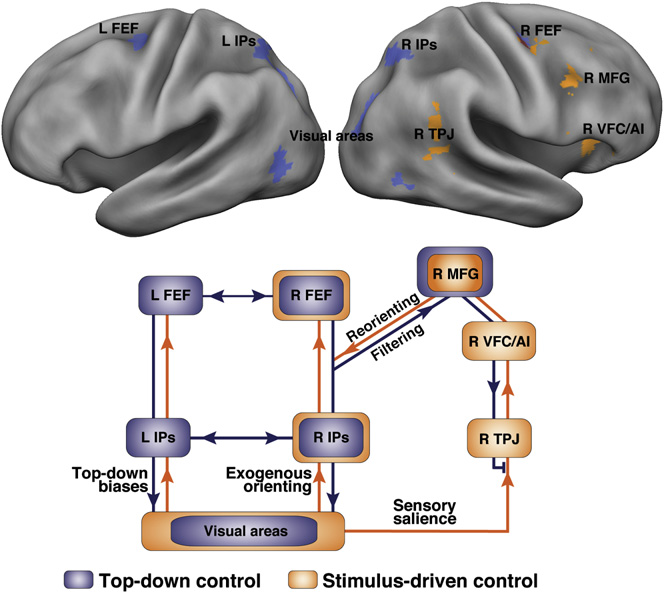
\includegraphics[scale=0.4]{img/attentionnetworks.png}
	\caption[Dorsal and ventral attention networks]
	{\small{Definition of dorsal and ventral networks from activation data, and putative interactions. Taken from \textcite{corbetta2008reorienting}.}}
	\label{fig:Networks}
\end{figure}



A core part of the dorsal attention system is the FEF. In humans, the FEF is located bilaterally in the rostral bank of a portion of the precentral sulcus at the caudal end of the middle frontal gyrus (see \ref{fig:FEF_reg}). Early insights about its function stem from stimulation studies with primates and were related to the FEF functions in the generation of eye-movements. These studies found an involvement of the FEF in almost all types of oculomotor events: Saccades (rapid movements of the eye between fixation points), fixations (maintenance of gaze), smooth pursuits (tracking of moving objects) and vergence movements (eye rotations necessary for bifoveated vision at differing target depths) (see \textcite{krauzlis2014eye} for an overview). The early works of Ferrier in the end of the 19th century, and later works by Bruce and colleagues (1985) reported the major involvement of the FEF in saccade generation: Low-intensity electrical stimulation of the FEF in the bank of the arcuate sulcus in monkeys elicits saccadic eye movements directed contralaterally to the stimulated hemisphere (\cite{tehovnik2000eye}). \textcite{bruce1985primate} further found a first subdivision of the FEF when they showed that saccades elicited by stimulation at a particular region have a particular direction and amplitude, independent of the orientation of the eyes. The more medial the stimulation of the primate arcuate sulcus, the larger the saccadic amplitude gets (\cite{bruce1985primate}), thus revealing a gradient of saccadic amplitudes from lateral to medial sites of the FEF. Hence, the ventrolateral portion of the FEF is generating shorter saccades, while the mediodorsal portion is generating longer saccades. 

\begin{figure}[H]
	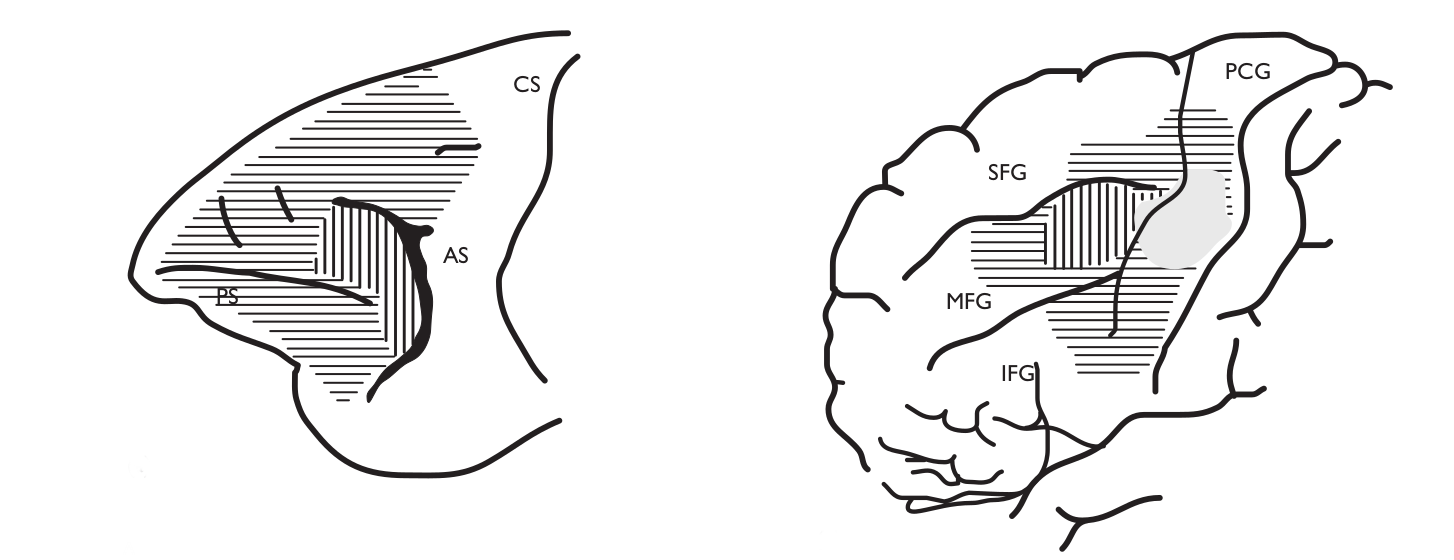
\includegraphics[scale=0.3]{img/FEF.png}
	\caption[Anatomical location of the FEF]{\small{Locations in monkey (left) and human (right) at which electrical cortical stimulation evokes eye-movements. Different shading corresponds to different studies. Taken from \textcite{blanke2000FEF}.}}
	\label{fig:FEF_reg}
\end{figure}

More recent stimulation studies in primates and high resolution fMRI experiments in humans further revealed that the FEF also contains zones that are involved in the control of other types of eye movements: Stimulation of the frontal pursuit-zone in the fundus elicits pursuit eye movements directed ipsilateral to the stimulated hemisphere (\cite{blanke2003direction}). The intracortical stimulation of several subareas within the FEF, among others a region within the pre-arcuate cortex in rhesus monkeys, rostral to the saccade related area, triggers vergence movements and is involved in accommodation (Crosby et al., 1952, cited by \textcite{vernet2014corrigendum}). Finally, the FEF is further active in the disengagement from fixations prior to a new saccade (\cite{goodwin2007cranial}; \cite{tehovnik2000eye}). They therefore play a crucial motor function in the major types of eye movements, most prominently saccades, but also pursuit, fixation, and vergence movements. \newline
Beyond its role in the control of gaze however, as its involvement in the dorsal attention network suggests, the FEF is further involved in aspects of higher cognition. The most compelling evidence stems from lesion studies: In monkeys, unilateral damage to the FEF results in contra-lateral neglect (\cite{crowne1981effects}), and temporary medically induced FEF inactivation delays and disrupts performance in covert visual search tasks, i.e. tasks that do not involve eye movement (\cite{monosov2009frontal}). In the same vein, FEF stimulation with electrical sub-threshold currents facilitates performance in change detection tasks: In a study by \textcite{moore2004microstimulation}, monkeys had to detect luminance changes of a target in the presence of salient, flashing distractors. Early electrical stimulation (250ms after stimulus onset) improved task performance in a similar magnitude to that of distractor removal. \newline Despite the partial dissociation of motor and attention functions of the FEF seen in covert attention (\cite{vossel2014dorsal}) and the possibility to disrupt it as shown by \textcite{monosov2009frontal}, attentional processes and motor functions of the FEF seem closely related. The convergence of functional and anatomical connections to both the visual system (\cite{stanton1995topography}, \cite{schall1995topography}) and the attention system (\cite{corbetta2002control}) underlines this. One hypothesized role for the FEF combining attentional and motor functions lies in holding a salience map that determines saccadic targets (\cite{itti2001computational}). \textcite{thompson2005visual} studied the FEFs role in saccade target selection in primates performing a visual search task. They found evidence for the existence of a heatmap-like representation of saliency encoded in selective activation that is related to the overall behavioral relevance of visual stimuli. This representation, the authors argue, arising from an integration of both top-down and bottom-up influences, then determines targets for foveation in the visual field in a 'the-winner-takes-it-all' fashion \textbf{gunnar sagt mehr erklärung hierzu}. Despite this proposed integrating role between attentional information, a majority of reported FEF activity appears to be in conjunction with endogenous attention. TMS studies over the FEF report larger deficiencies or larger latencies in saccadic movements with a voluntary component (e.g. after endogenous cues), but only mild effects on reflexive saccades (usually using more exogenous paradigms such as briefly flashed visual targets) (\cite{vernet2014corrigendum}). In healthy humans, \textcite{muggleton2003human} found repetitive transcranial magnetic stimulation (rTMS) at 10Hz for 500ms to interfere only with those subtypes of visual search involving endogenous attention, namely where a visual target is neither salient nor predictable. And \textcite{grosbras2002transcranial}in the same vein found an effect of TMS in an attention task involving endogenous attentional deployment. Apart from a differential involvement in endogenous versus exogenous attentional processes, a number of studies also reveal hemispheric differences in the attentional functions of the FEF. For one, in the broader context of attention networks, neuropsychological patient studies find attentional deficits such as visuo-spatial neglect more often after right-hemispheric than left-hemispheric brain damage (\cite{vernet2014corrigendum}), and affected patients show deficits in saccade planning to the left hemisphere (\cite{Behrmann2001ImpairedIB}). One hypothesis for this observation concerns the right-hemispheric dominance of the ventral attention system\footnote{While there is some differential evidence for the TPJ (see \textcite{vossel2014dorsal}, for a short overview) a majority of studies showed a lateralization of the ventral system to the right hemisphere (\cite{corbetta2002control}; \cite{fox2006spontaneous}; \cite{corbetta2008reorienting}).}. In its interaction with the dorsal attention system (\cite{he2007breakdown}) through the superior longitudinal fasciculus, ventral network lesions can lead to the saccadic deficits common in neglect (\cite{friston2018neglect}). A recent study by \textbf{Meyer et al (2018)} explored whether hemispheric differences between endogenous and exogenous attention can be found  in the dorsal attention network. They found an interaction between hemisphere, attention mode, and brain region, with the left frontal eye fields being selectively more activated than parietal regions during endogenous conditions \textbf{this does not make sense yet}. Studies within the FEF alone also find hemispheric differences. The aforementioned TMS studies of  \textcite{muggleton2003human} and \textcite{grosbras2002transcranial}both found effects during stimulation over the right FEF, but not the left FEF. Lastly, a location closely connected to the FEF and also involved in the generation of saccades and attentional deployment, the intraparietal sulcus (IPS), was found to display differences in visual field representation between hemispheres depending on attentional modulation (\cite{sheremata2015hemisphere})\textbf{what does this mean???}.\newline
In conclusion, the frontal eye fields are an interesting structure occupying important roles in eye movements, aspects of higher cognition, in particular visuospatial attention, and their interaction. Following the reasoning of \textcite{vernet2014corrigendum} and the short overview given in this section, studies of the frontal eye field in conjunction with the cognitive context during activation could shed light on how attentional processes modulate the activation of the FEF. Given the evidence for some hemispheric differences outlined above, this question can be extended to the differences in left and right FEF activation given different attentional modulation.
In this thesis, therefore, it will be explored whether activation differences in the left and right frontal eye field can be explained by exogenous and endogenous attentional modulation. \textbf{And now we need a clearly stated research question and ideally some hypothesis} Based on the findings that right FEF inhibition disrupts endogenous attentional tasks in particular (\cite{muggleton2003human}; \cite{grosbras2002transcranial}), it is hypothesized that a stronger endogenous attentional mode will be differentially related to higher activation in right FEF. \textbf{why would these findings help the world}\newline
\textbf{lets do another thesis overview here, just to be safe :D} \\
\textbf{finally add an outro that state something that gets us back to the visuospatial attention system}

\textbf{maybe include:}
\begin{itemize}
	\item http://sci-hub.tw/https://www.sciencedirect.com/science/article/pii/S0028393218300630: A recent study by Meyer et al (2018) studied hemispheric differences in the frontal eye fields an the intraparietal sulcus (IPS) between exogenous and endogenous attention conditions of a visual discrimination task... OR explored whether differences between endogenous and exogenous attention in the dorsal attention network can be found... They found an interaction between hemisphere, attention mode, and brain region, with the left frontal eye fields being selectively more activated than parietal regions during endogenous conditions... The dorso-frontal attention network is associated with both types of attentional orienting, but the type of attention differentially engages the network over time and across hemispheres
	\item The Sheremata paper with larger perceptual fields
\end{itemize}


\subsection{Studying of visuospatial attention with complex stimulation }
Visuospatial attention is usually studied by means of highly controlled experimental tasks, such as Posners' cueing paradigm (\cite{posner1980attention}) or simple visual search tasks. While well controllable, these conventional laboratory experiments suffer from a lack of ecological validity and fail to evoke realistic competing demands for visuospatial attention. As \textcite{hasson2004intersubject} noted, controlled experimental settings bear little resemblance to natural viewing for at least four reasons: 1) Lack of complex visual scenes (i.e. presentation of visual stimuli in isolation), 2) Lack of (complex) movement, 3) Lack of unconstrained eye movement, and 4) Lack of interactions between vision and additional modalities, context and emotional valence. Naturalistic stimulation such as watching movie clips, in contrast, does not suffer from these shortcomings. Therefore, while static images have been an object of interest in the analysis of gaze distribution and attention from the early works of \textcite{yarbus1967eye} onwards, movies or videos became a promising stimulus choice during the past decade: They contain interesting, multisensory stimuli and are more representative of natural vision arrays than static pictures. As movie content constantly changes and includes both salient elements such as motion, as well as top-down components from the attempts to comprehend and interpret the content (\cite{ross2013eye}), movies represent an ideal possibility to study the dynamic and complex interplay of attentional processes ecologically valid (e.g. in \textcite{hasson2004intersubject}; \cite{carmi2006visual}; \cite{tseng2009quantifying}; \cite{dorr2010variability}).

An open, neuroscientific dataset that contains a variety of measures obtained during naturalistic stimulation is the studyforrest project (http://studyforrest.org/). A large portion of the data that is provided in this project is used for the purpose of this thesis. As the following general method section will outline, it contains both functional and behavioral data in the form of eye tracking, and thus bears the interesting chance to study of the FEF as a structure involved in motor tasks in the movements of the eye and higher cognitive aspects of visuospatial attention on both of these dimensions. \textbf{outro sentence here}



\section{General methods}\label{section:generalmethods}

This section introduces the common data basis, general preprocessing steps, and the software the analyses rely upon. Any additional analysis-specific methodological information is stated in the respective chapters' method sections.

\subsection{Data basis}

Data for all analyses stems from the 2016 released extension of the studyforrest dataset\footnote{All data and code are publicly available at https://github.com/psychoinformatics-de/studyforrest-data-phase2.} (\cite{hanke2016studyforrest}; \cite{sengupta2016studyforrest}). In this extension, $N = 15$ right-handed participants (age range 21 – 39 years, mean age 29.4 years, six female, normal or corrected-to-normal vision), who had previously participated in the studyforrest project, watched the audio-visual movie “Forrest Gump” (R. Zemeckis, Paramount Pictures, 1994) during simultaneous fMRI and eye-tracking recording. They further underwent a traditional localizer paradigm for higher visual areas: The fusiform face area (FFA), the occipital face area (OFA), the extrastriate body area (EBA), the hippocampal place area (PPA), the lateral occipital complex (LOC) and early visual cortex (\cite{sengupta2016studyforrest}).

\subsection{Stimulus material}

Stimulus material for the audiovisual movie was the German dubbed version of Forrest Gump (Zemeckis, Paramount Pictures, 1994). The video track for the movie stimulus was re-encoded from Blu-ray into H.264 video (1280 x 720 at 25 frames per second (fps)). In accordance to the procedure in an earlier phase of the studyforrest project, the movie was shortened by removing a few scenes less relevant for the major plot to keep the fMRI recording session under two hours. The shortened movie was then segmented into eight segments of roughly 15 minutes of length (for an overview on segment duration, final stimulus content and detailed procedures see \textcite{hanke2014high}). Stimulus material for the localizer paradigm consisted of 24 unique gray-scale images for each of six different categories (faces, bodies, houses, scenes, everyday objects, and scrambled images) at a resolution of 400 x 400px, matched in luminance, and displayed at 10 x 10$^\circ$ of visual angle (\cite{sengupta2016studyforrest}). 

\subsection{Procedures}
Functional MRI data acquisition for the audio visual movie was undertaken in two consecutive recording sessions on the same day, with a break of flexible duration. Within each session, four movie segments were presented in chronological order (\cite{hanke2016studyforrest}). Visual stimuli were projected on to a screen inside the bore of the magnet using an LCD projector, and presented to the subjects thought a front-reflective mirror on top of the head coil at a viewing distance of 63cm. The screen dimensions were 26.5cm x 21.2cm (corresponding to 1280 x 1024px) at a resolution of 720p at full width, with a 60Hz video refresh rate (\cite{sengupta2016studyforrest}). Eye-tracking was performed with an Eyelink 1000 (software version 4.594) using monocular corneal reflection and pupil tracking with a temporal resolution of eye gaze recordings of 1000Hz. The camera was mounted at an approximate distance of 100cm to the left eye of subjects, which was illuminated by an infrared light source (\cite{hanke2016studyforrest}). Movie presentation and eye-tracking were synchronized by starting the eye gaze recording as soon as the stimulus computer received the first fMRI trigger signal. Timings of subsequent trigger pulses and onsets of every movie frame were logged. Using a 3 Tesla Philips Achieve dStream MRI scanner with a 32 channel head coil, T2*-weighted echo-planar images (gradient-echo, TR = 2s, echo time = 30ms, flip angle = 90) were acquired during movie watching. For the eight segments, 451, 441, 438, 488, 462, 439, 542, and 338 volumes were acquired, respectively (\cite{hanke2016studyforrest}). Eye-tracking data were normalized such that all gaze coordinates are in native movie frame pixels, with the top-left corner of the movie frame located at (0, 0) and the lower-right corner located at (1280, 546) (\cite{hanke2016studyforrest}). The amount of unusable data, primarily due to signal loss during eye blinks, ranged from less than 1 to 15\% for 13 of the 15 in-scanner subjects (the other two subjects’ data contained 85 and 36\% of data loss, respectively). In-scanner acquisition had an approximate spatial uncertainty of 40px according to the calibration procedure (\cite{hanke2016studyforrest}).\newline

In the localizer paradigm, participants viewed the different object categories in a total of four block-design runs, with two 16s blocks per stimulus category. The order of the individual images per category differed across runs and participants, but the sequence of category blocks was the same for every run and participant. Localizers for higher visual areas (FFA, OFA, PPA, LOC, EBA, and early visual cortex) were obtained by the original authors of the studyforrest extension with a two-level GLM analysis on contrasts of activation between object categories (for details, see \cite{sengupta2016studyforrest}).

\subsection{Software}
Data preprocessing and analysis were conducted with a multitude of Python-based software packages. Preprocessing of data relied primarily on custom made workflows written with nipype (\cite{gorgolewski_krzysztof}), and utilizing FSL (\cite{jenkinson2012fsl}). Much of the data analysis used using PyMVPA (\cite{hanke2009pymvpa}). Datalad (\cite{visconti_di_oleggio_castello_matteo_2019_2560733}), a version control tool for scientific data, served as a backbone for all own work presented in this thesis. Datalad-container (\cite{michael_hanke_2018_2431915}) was used during preprocessing. If applicable and unless otherwise stated, the alpha level for statistical significance was set to $\alpha = 0.05$.

\subsection{Preprocessing of fMRI data}

Motion-corrected fMRI data in subject-space were obtained from the respective Github repositories via datalad (\cite{visconti_di_oleggio_castello_matteo_2019_2560733}). In a first step, both localizer and movie-data fMRI datasets, were preprocessed identically using a custom made nipype workflow, consisting of whole-brain masking, high-pass filtering with a cutoff of 50Hz, and smoothing with a Gaussian kernel of 4mm FWHM\footnote{All code for preprocessing and analysis can be found at https://github.com/AdinaWagner/localizer.}. Subsequently, all data were warped into a study-specific group template using FSL (\cite{jenkinson2012fsl}). 




\chapter{A novel method for determining functional ROI specificity}\label{c1}

Most research paradigms in neuroscience employ highly controlled stimulation protocols with subsequent contrasts in a GLM to precisely pinpoint and disentangle the function or location of the structure in question (\cite{Kanwisher11163},  \cite{fox2009defining}). For example, to localize higher visual areas, \textcite{sengupta2016studyforrest} employed a six category block-design (faces, houses, bodies, scenes, objects, scrambled images), and contrasted the activation during certain category conditions with the activation during others. However, this approach may not be optimal. 
First, the employed artificial stimulation is not ecologically valid, which decreases the sensitivity of functional localizers and thus their applicability across studies. \textbf{TODO: This needs an example or citation} Secondly, a reliance on narrow stimulus categories and simple contrasts omits insights into further stimulus aspects of potential relevance - especially since an exact contrast between conditions accounting for various ROI-specific factors is rarely known ahead of time, and thus cannot be incorporated into the localizer GLM contrast. While well-studied ROIs are known to be differentially activated by certain stimulus features, their response to other stimulus features may not be understood completely. Likewise, while certain contrasts are established in the differentiation of ROIs (e.g. faces versus houses), it is not clear whether this contrast is distinguishing the ROIs with highest precision, or whether other contrasts would improve the differentiation. \textbf{TODO: This would also benefit from an example/citation} Lastly, it is challenging to differentiate functionally related but different ROIs with a simplistic experimental design and coarse stimulation categories. As such, localization often requires subsequent segregation of clusters based on spatial coordinates and known anatomical location of the ROI in question (such as the OFA and the FFA; see e.g \cite{sengupta2016studyforrest}).
Obtaining additional insights with regard to the functionality of regions of interest might be beneficial to reduce reliance on spatial information, improve future models used in localization paradigms, and may additionally give new insights into the functional neuroanatomy of ROIs.\newline
In the first chapter of this thesis, based on these shortcomings, I will outline a novel approach to determine the functional specificity of functional ROIs. The method is designed to estimate a maximally discriminative contrast between the functional signatures of any two ROIs in question, and to use the available information about anything about the experimental design - regardless of complexity - to provide a functional description for it. The results of this analysis should give differential insights into the functional specificity of ROIs beyond simple contrasts of stimulus conditions, and thus provide a method to study the influence of attentional modes evoked by a movie stimulus on the FEF. \newline
The method combines a classification analysis with a subsequent GLM computation. This second step relies on \textit{sensitivity profiles} derived during the classification analysis. A short introduction into the basic principles of this type of machine learning tool and and the chosen algorithm for this analysis will be introduced in the next subsection, followed by an elaboration on how the derived sensitivities are further utilized. In order to validate the method, its applicability and generalization capabilities were first tested on a general localization paradigm, and later movie-data, for already localized ROIs, which will be elaborated on in section \ref{c1:methods}.


\section{Overview}
The general idea behind the proposed method is to derive a functional signature as the parameter vector describing a linear decision boundary between two ROIs in question, and to explain this functional signature by providing a detailed description of the experimental design. This is realized with a two step procedure consisting of (1) \textit{classification} and (2)\textit{ GLM analysis}.  In the first step, the classification, voxel are classified into ROIs in a leave-one-out cross-validation. This classification step is a replication of a \textcite{nastase2016} and serves as a vehicle for a simultaneous sensitivity analysis to derive the parameters of the hyperplane that describe the decision boundary between all pairwise ROI classification decisions. In the second step, the GLM, the obtained timecourse of sensitivities is modeled with the available experimental design. Importantly, the method relies on transposing the fMRI dataset, such that all time points are features, and the voxels are samples. The following subsections elaborate on these steps. \newline


\subsection{Step 1: Classification analysis}
The term \textit{classification analysis} is most often used in the context of \textit{machine learning}. Machine learning refers to the study and construction of software that can learn from data without being explicitly programmed (\cite{zeigermann2018machine}). Especially in the data-rich environment of neuroimaging, machine learning algorithms and techniques have gained immensely in popularity and significance as for their ability to detect hidden patterns and trends in the data (\cite{vogt2018machine}). One particular type of tool from machine learning is a so called \textit{classifier}, which is used for a classification analysis. In such an analysis, a classifier is trained on a subset of data, the \textit{training set}, and is then used for predictions on a previously unseen subset of data, the \textit{test set} (\cite{zeigermann2018machine}). \newline
More formally, a classifier is a function created from training data to predict the value of a class attribute $C \in \{1, \ldots, r\}$ (the \textit{label}), given the predictive \textit{features} $X = (X_1, \ldots, X_d)$  with values in $S = \{S_1 \times \ldots \times S_d\}$ and the sample $x = (x_1, \ldots, x_d)$. Suppose $(X, C)$ is a random vector with a joint feature-label probability distribution $p(x, c)$. A classifier $\psi$ is the function that maps X onto C:

\begin{equation}\label{classifier}
\psi:\{ S_1, \times \ldots, \times S_d \} \rightarrow \{1, ..., r\}
\end{equation}
\begin{equation}
x \mapsto c.
\end{equation}


The overall aim of the classification analysis in this thesis was not the classification in general, but to derive a sensitivity measure in the form of feature weights from a simultaneous sensitivity analysis. Even though the overall problem is a (potential) multiclass classification, i.e. samples are classified into three or more classes, to derive such sensitivities, the classification in transformed into multiple binary 1-vs-1 classifications. The choice of classifier for this thesis aims to yield an interpretable, linear hyperplane as the decision boundary between each two classes. \newline
There are a number of different classification algorithms available to build classification models. Based on prior work of \textcite{nastase2016}, a \textit{linear Gaussian Naive Bayes} classifier (GNB) was further explored due to its high classification accuracy and easy interpretability of feature weights. Additionally, a \textit{Stochastic Gradient Descent} algorithm was used to validate the consistency of results obtained with the GNB, but will not be elaborated on further. Section \ref{sec:c1_cv_res} will show the high similarity in the results between both classifiers. \newline
The GNB algorithm belongs to the family of Naive Bayes algorithms. These algorithms use a probabilistic approach to classification, utilizing the Bayes theorem to capture the relationships within input data and output label. Given some samples $x_1, \ldots, x_n$ with a number of characteristics on different features, and labels $c_1, \ldots, c_r$, naive Bayes classifiers learn a model of the joint probability, $p(x, c)$ during training. During testing, they make predictions by using Bayes theorem to calculate the probability of a label, given the feature characteristics of a sample, $p(c|x)$. Two fundamental assumptions exist for these algorithms: \newline 
\begin{itemize}
	\item \textit{Conditional independence}: Each feature $x_i$ is independent of every other feature $x_j$ for $j \neq i$ given the outcome $c_r$.
	\item \textit{Equal contribution of features}:  Each feature is given the same weight for the outcome prediction. 
\end{itemize} 
A linear Gaussian Naive Bayes classifier further assumes the data to be distributed according to a Gaussian distribution, and it assumes the feature variance to be independent of class (i.e. $\sigma_{i, 0}^2 = \sigma_{i, 1}^2$). Given the latter assumption holds, the decision boundery between any two classes 1 and 0,
\begin{equation}
\prod_{i=1}^{d} P(X_i |C = 0)P(C=0) = \prod_{i=1}^{d} P(X_i |C = 1)P(C=1),
\end{equation}
is linear (for the mathematical proof, see e.g. \textcite{DBLP:books/daglib/0087929}), chapter 3). The feature weights of this classifier are defined as
\begin{equation}
w_i = \sum_{i}\frac{\mu_{i, 0}-\mu_{i, 1}}{\sigma_{i}^{2}}.
\end{equation}


Figure \ref{GNB} illustrates the case of two features and two classes with their respective distribution. The feature weight of the feature $A$ can be derived as the difference in means given the class, $\mu_{A, 1} - \mu_{A, 2}$, divided by their common variance. In the displayed example, Feature A with a feature weight close to zero has little value for the differentiation of the classes, whereas feature B is highly informative. \newline

\begin{figure}[H]
	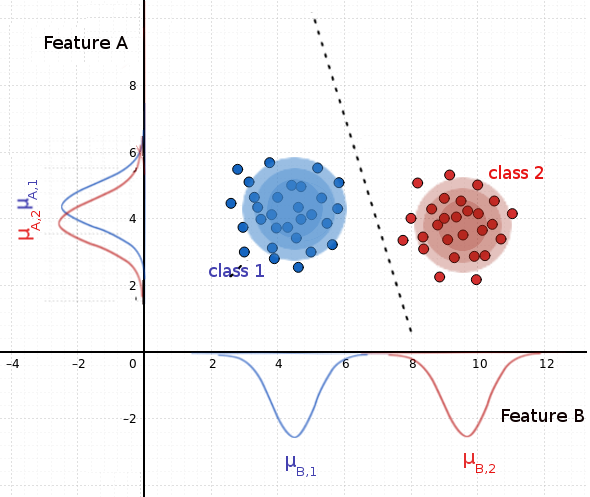
\includegraphics[scale=0.5]{img/improved_GNB.png}
	\caption[A linear decision boundery for a linear Gaussian Naive Bayes classifier]{\small{Exemplary illustration of a linear decision boundary in the case of equal variances. The distribution of each features data given the class follows a Gaussian distribution with mean $\mu_i$ and variance $\sigma^2$.}}
	\label{GNB}
\end{figure}

To summarize, the linear Gaussian Naive Bayes classifier treats each feature independently and does not involve internal feature weighting or selection  \textbf{TODO:why is that a good thing?}. Furthermore, its decision boundary hyperplane parameters have a straightforward interpretation, especially in the case of a transposed dataset, as the next section will show.
\bigskip


\noindent \textbf{A "transposed" approach to the functional sensitivity of ROIs}\hfill
\medskip

The method utilizes the sensitivites obtained during a classification analysis and thus extends work by \textcite{nastase2016}: Following a classification of voxels (samples) to ROIs (labels) based on the observed data in the ROIs from other participants, a subsequent analysis of the classifiers sensitivity profile obtained from a decision between ROI pairs is used to shed light onto their functional distinctiveness. One crucial step in the computation lies in transposing the dataset. As opposed to the common approaches at classification with subsequent sensitivity analysis in neuroimaging (e.g. as used in \textcite{poldrack2009decoding}), transposing the datasets makes features in this classification problem \textit{time points}, while \textit{voxels }constitute samples. Thus, during classification, voxels are classified into ROI labels based on their activation at different time points. \newline
This approach holds two advantages: For one, it enables the classification of voxel to ROIs in the first place. In the first analysis step, the functional signature of ROIs is obtained from a classifiers' sensitivity profile in an n-fold leave-one-participant-out cross-validation: The classifier is trained on all subjects except for one and then tested on that out-of-sample individual, and this method is repeated for each of the subjects. The cross-validation approach further allows an estimation of the generalization performance of the classification. Secondly, in the case of a linear GNB algorithm, the feature weights are easily interpretable. As the dataset is transposed to have time points as features, this functional signature is a time course of sensitivities, and each weight corresponds to the difference in mean activation of all voxels given the label (ROI) at one time point, normalized by their common variance. In an examplary decision between ROIs 'class 1' and 'class 2', a negative weight as for time point B corresponds to an overall higher activation in class 2 at this particular point in time. Such sensitivity time courses are computed for all pairwise combinations of classes. The obtained sensitivity profile vectors per fold of the cross-validation are averaged across folds, and normalized by their L2 norm. As a result, there is one temporal sensitivity profile for each pairwise ROI combination. The achieved overall classification accuracy serves as a measure of whether population wide functional specificity and sensitivity between the ROIs can be captured. An exemplary time course of sensitivities for the FFA and PPA during a block stimulation is depicted in the black line in \ref{fig:tc}. The figure further contains two activation time courses for two random voxels of the FFA (blue) and PPA (red). \newline

\begin{figure}[H]
	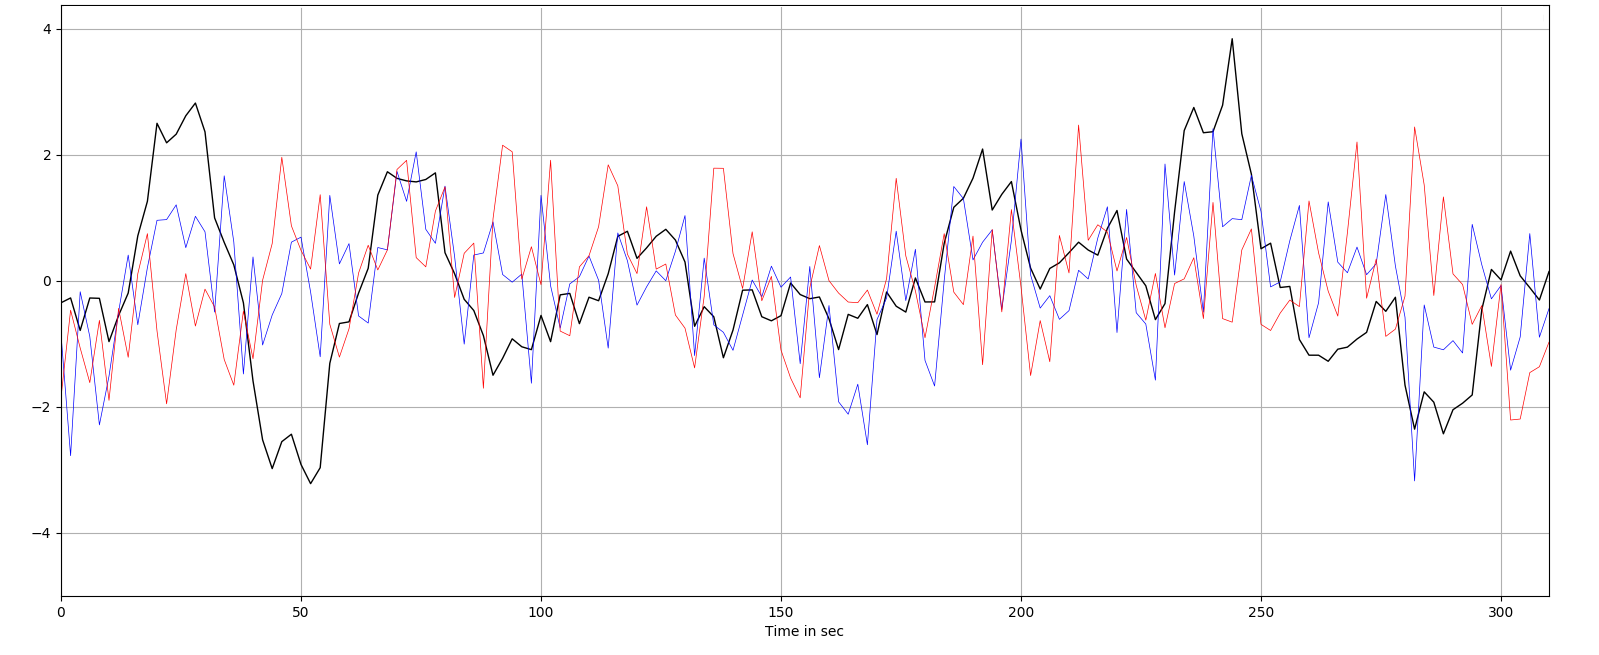
\includegraphics[scale = 0.37]{img/tc_loc_plusvox_v2.png}.
	\caption[Examplary time course of sensitivities]{\small{Sensitivity time course of two ROIs, the FFA and PPA, during a standard localizer block design. Blue and red graphs are activation profiles of a random FFA (blue) and PPA (red) voxel over the same time span. The figure serves illustrative purposes only, and will be shown completely in section \ref{section:c1_results}}}
	\label{fig:tc}
\end{figure}

\subsection{Step 2: GLM}

The subsequent GLM builds up on the sensitivity analysis during classification. To obtain insights into the stimulus features driving the activation differences between ROIs in question, the available experimental design is transformed into regressors, convolved with an HRF, and used to model the sensitivity profile. The resulting coefficients indicate the importance for each regressor (i.e. stimulus characteristic) for the distinction between ROIs. Section \ref{c1:methods} will give a comprehensive example of this approach. As the datasets are transposed prior to the classification analysis to have time points as features, in the case of the GNB, each weight corresponded to the normalized difference in mean activation of all voxels given the class at one time point. In case of for example the decision between FFA and PPA, a negative weight therefore corresponds to an overall higher PPA activation at this particular point in time. The type of stimulation present at this point in the experimental design likely contributes to the distinction between the two areas, and the magnitude of its influence will be visible in its associated beta coefficient obtained from the GLM.
	

\section{Methods}\label{c1:methods}
In order to establish feasibility of the procedure and to test the generalization of the developed approach, the method was validated in a two-step procedure. As a test of plausibility, it was used on data from a standard block design for ROI localization within the studyforrest dataset. As a measure of its capabilities to generalize to naturalistic stimulation, it was subsequently used with the studyforrests' movie data, collected on the same participants. For both datasets, six functional ROI masks (FFA, PPA, OFA, EBA, LOC, early visual cortex) were available to serve as labels during classification analysis. Both validating analyses were restricted to the well-explored and functionally distinct ROIs FFA and PPA as for the wealth of literature concerned with these ROIs.  
All code used in this analysis can be found on Github\footnote{https://github.com/AdinaWagner/localizer}. 

\subsection{Analysis-specific data}

Data consists of the custom preprocessed localizer and avmovie datasets with the accompanying ROI masks (see section \ref{section:generalmethods}). For illustrative purposes, figure \ref{fig:stims} shows one example image per category used in the localizer paradigm.

\begin{figure}[H]
	\subfigure{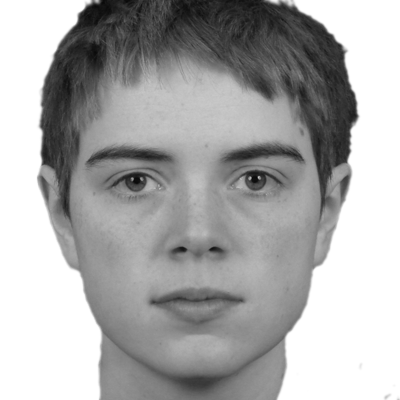
\includegraphics[width=0.15\textwidth]{img/face01.png}}
	\subfigure{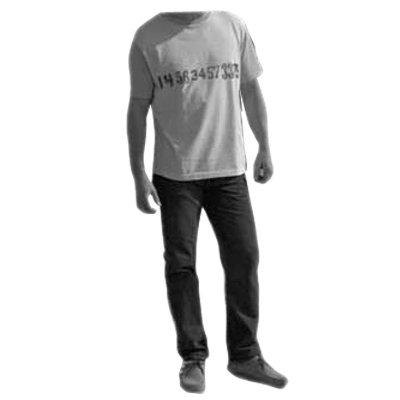
\includegraphics[width=0.15\textwidth]{img/body01.png}}
	\subfigure{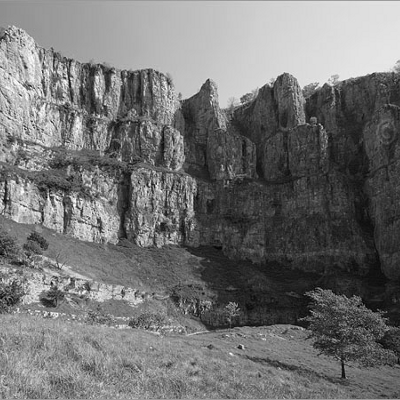
\includegraphics[width=0.15\textwidth]{img/scene01.png}}
	\subfigure{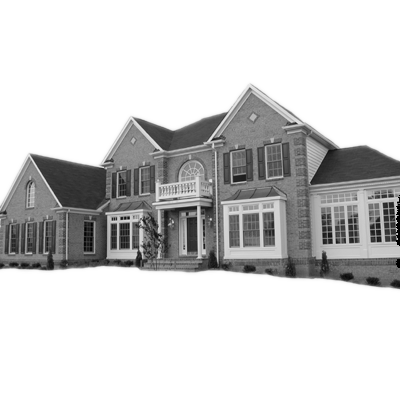
\includegraphics[width=0.15\textwidth]{img/house01.png}}
	\subfigure{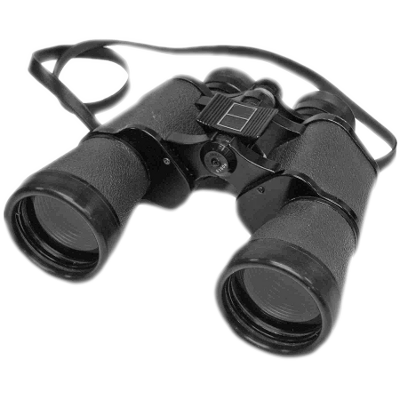
\includegraphics[width=0.15\textwidth]{img/object01.png}}
	\subfigure{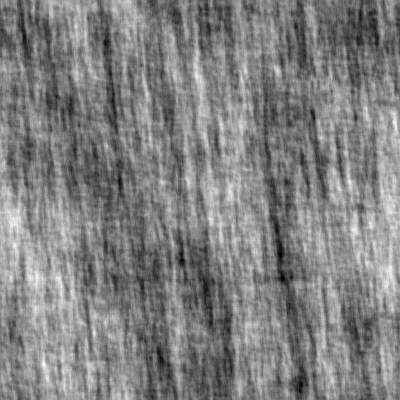
\includegraphics[width=0.15\textwidth]{img/scramble01.png}}
	\caption{\small{Image categories used for localization.}}
	\label{fig:stims}
\end{figure} 

In addition to the aforementioned data, the method requires information about the experimental paradigm or the stimulation. For this purpose, for the localizer data analysis, the stimulation event files from the block-stimulation were obtained from the public repository\footnote{https://github.com/psychoinformatics-de/studyforrest-data-visualrois}. The dynamic, naturalistic nature of the movie did not permit any experimental design description, but several annotations of the movie were used instead: The location annotation by \textcite{hausler2016annotation}, providing a detailed description of a scenes' setting in different levels of abstraction as well as onset and duration information, and an automatic feature extraction using Google's Cloud Vision API via the pliers toolkit (\cite{yarkonipliers}), providing frame-wise counts of faces. 


\subsection{Preprocessing}

For use in the localizer dataset, the event files describing the stimulation protocol of the object-category task were used to compute a group-level event file. This was possible because the order of blocks was the same across runs and participants (see \cite{sengupta2016studyforrest}). For each participant, the onsets of each image were averaged. Deviations from individual onsets to the average group onsets were smaller than 0.5 seconds. In addition to the six object categories, the first occurrence of an image within an object category was classed a new type of event with the suffix 'first', resulting in 12 regressors (face, face\_first, body, body\_first, house, house\_first, scene, scene\_first, object, object\_first, scramble, scramble\_first). This was done to account for any additional variation introduced by a sudden change in categories. 
For generalization in the movie dataset, the available annotations were transformed into events. An event was derived for each "setting" in the location annotation occurring more than once. An event was further derived for night-time, a scene being located exterior, a cut to a new scene, and contextual jumps to future or past from the previous shot. The facial feature data was downsampled to seconds and two conditions were derived, "face" for any one second time window with a maximum of less than 3 faces, and "many\_faces" for any one second time window with 3 or more faces present.
For both analyses, the resulting events are convolved with an HRF and entered as regressors to explain the time course of sensitivities using PyMVPAs (\cite{hanke2009pymvpa})  \texttt{fit\_event\_hrf\_model() }function. \newline

\subsection{Required software implementations}

Both classifiers of choice were readily available in PyMVPA (\cite{hanke2009pymvpa}). The Gaussian Naive Bayes classifier is implemented as \texttt{GNB()} and customizable to be a linear classifier with the parameter \texttt{common\_variance = True}. The Stochastic Gradient Descent classifier is imported from the Python module \texttt{sklearn} and wrapped with PyMVPAs \texttt{SKLLearnerAdapter()}. To enforce pairwise 1-vs-1 decisions, it is further wrapped with PyMVPAs \texttt{MulticlassClassifier()}. \newline
Both classifiers, however, lacked functionality to compute feature weights for a sensitivity analysis. Therefore, I extended the GNB class in the sourcecode of the pymvpa package with the implementation of the subclass \texttt{GNBWeights}\footnote{This contribution is already merged to be part of the pymvpa sourcecode}. For the MulticlassClassifier() and SKLLearnerAdaptor() used to wrap the SGD, I implemented the subclasses \newline \texttt{MulticlassClassifierSensitivity(BoostedClassifierSensitivityAnalyzer)} and  \texttt{SKLLearnerAdapterWeights(Sensitivity)}\footnote{At the time of thesis submission, this contribution is a pull request and can be found at: https://github.com/PyMVPA/PyMVPA/pull/596}. For both classifiers, this enables a sensitivity analysis that returns the classifier-specific weights for each feature for any possible pair of labels in a binary decision. As an example, consider a classification task with three labels L0, L1, L2, and two features, F1, F2. The implemented sensitivity analyzer will for each possible pair of labels (L0 versus L1, L0 versus L2, L1 versus L2) return one weight per feature. 

\subsection{Proof-of-Concept analysis}

For each the localizer and the movie data, a group dataset was build from the preprocessed BOLD data in group-space and the subject-specific ROI masks in group-space. Prior to the analysis, any overlap between ROIs was excluded from the datasets.
For both datasets, sensitivities were derived for the full dataset (including the ROI 'rest of the brain') and a stripped dataset consisting only of the six higher visual areas. For the proof-of-concept analysis, the ROIs were combined across hemispheres.  Each of these analyses were computed with a GNB and an SDG classifier. As regressors derived from the more complex annotation events are less intuitively understood, a coarse descriptive analysis of movie scenes associated consistently (i.e. across datasets and classifiers) with a high positive or high negative beta value was performed: The middle frame of the movie scene in question is extracted to gain superficial insights into the content of the scene. This part of the analysis is found in Appendix \ref{A:addons}.

\section{Results}\label{section:c1_results}

This section presents the results separately for each step of the method. Section \ref{sec:c1_cv_res} briefly outlines the results from the classification analysis, and section \ref{sec:c1_glm_res} presents the subsequent GLMs results.

\subsection{Classification results}\label{sec:c1_cv_res}

Table \ref{tab:CV} gives an overview of the classification accuracies achieved within the different analyses. 
Figure \ref{fig:CV} displays the classification confusion matrices for the localizer experiment and the movie experiment obtained from a classification of the stripped dataset with a GNB classifier.

\begin{table}[h!]
	\begin{center}
		\caption{Classification accuracies of the proof-of-concept analyses}
		\label{tab:CV}
		\begin{tabular}{l|c|c} % <-- Alignments: 1st column left, 2nd middle and 3rd right, with vertical lines in between
			\textbf{dataset} & \textbf{GNB} & \textbf{SGD}\\
			\hline
			Localizer dataset (with rest of brain) & 93.09 & 97.69\\
			Localizer dataset (without rest of brain) & 83.74 & 84.74\\
			Movie dataset (with rest of brain) & 91.0 & 95.46\\
			Movie dataset (without rest of brain) & 82.92 & 83.53 \\
		\end{tabular}
	\end{center}
\end{table}

As the classification results obtained with GNB and SGD are comparable despite the stricter assumption of the GNB, results are reported only for the GNB classifier due to its straightforward interpretation.

\begin{figure}[H]

	\subfigure{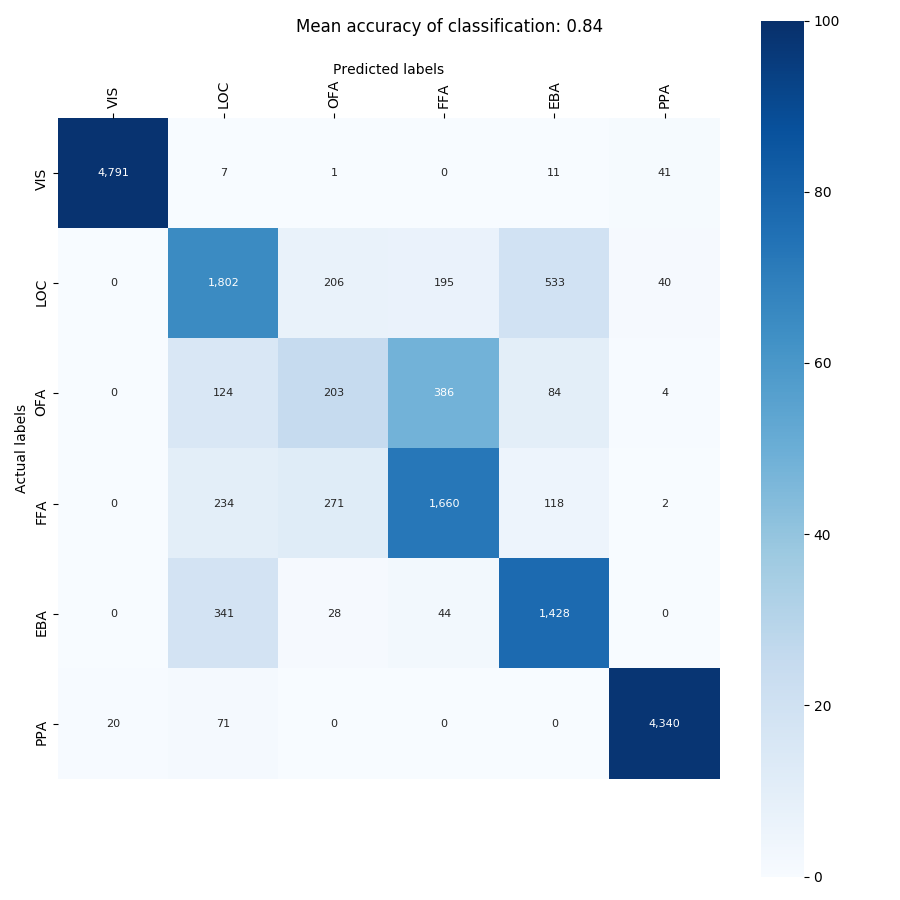
\includegraphics[width=0.49\textwidth]{img/CV_bilat_stripped_localizer.png}}
	\subfigure{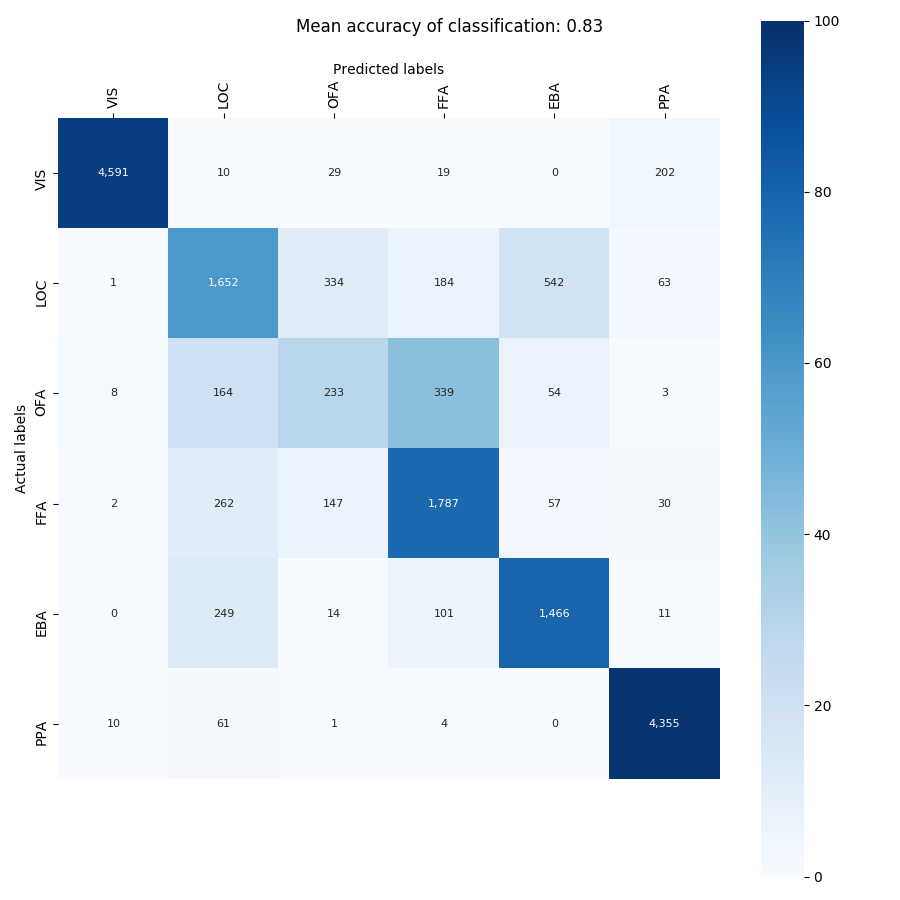
\includegraphics[width=0.49\textwidth]{img/CV_bilat_stripped_avmovie.png}}
	\caption[Classification results in two proof-of-concept analyses]{\small{Confusion matrices of ROI classifications across subjects in the localizer (left) and movie (right) experiments. Color shows classification accuracy (from 0 to 100$\%$) while numbers in each cell correspond to the actual number of voxels across all subjects }}
	\label{fig:CV}
\end{figure}




\subsection{GLM results}\label{sec:c1_glm_res}

Figure \ref{fig:locsens} shows the results of both GLM analysis: The graph depicts the time course of sensitivities (black) and the corresponding GLM fit (red) for the localizer experiment (top panel) and the movie data (bottom panel B) for the first run of each of these experiments with sensitivities derived from classification with a GNB algorithm for the ROIs FFA and PPA. For the localizer dataset, the GLM fit amounts to $R^2 = .90$. For the movie experiment, the fit is substantially lower with $R^2 = .26$. The stimulus features (regressors) yielding a differentially higher FFA activation have positive beta weights (localizer dataset: Body, face, and object related regressors), while those yielding differentially higher PPA activation have negative beta weights (localizer dataset: scene, house, scrambled images related regressors).

\begin{figure}[H]
	\subfigure{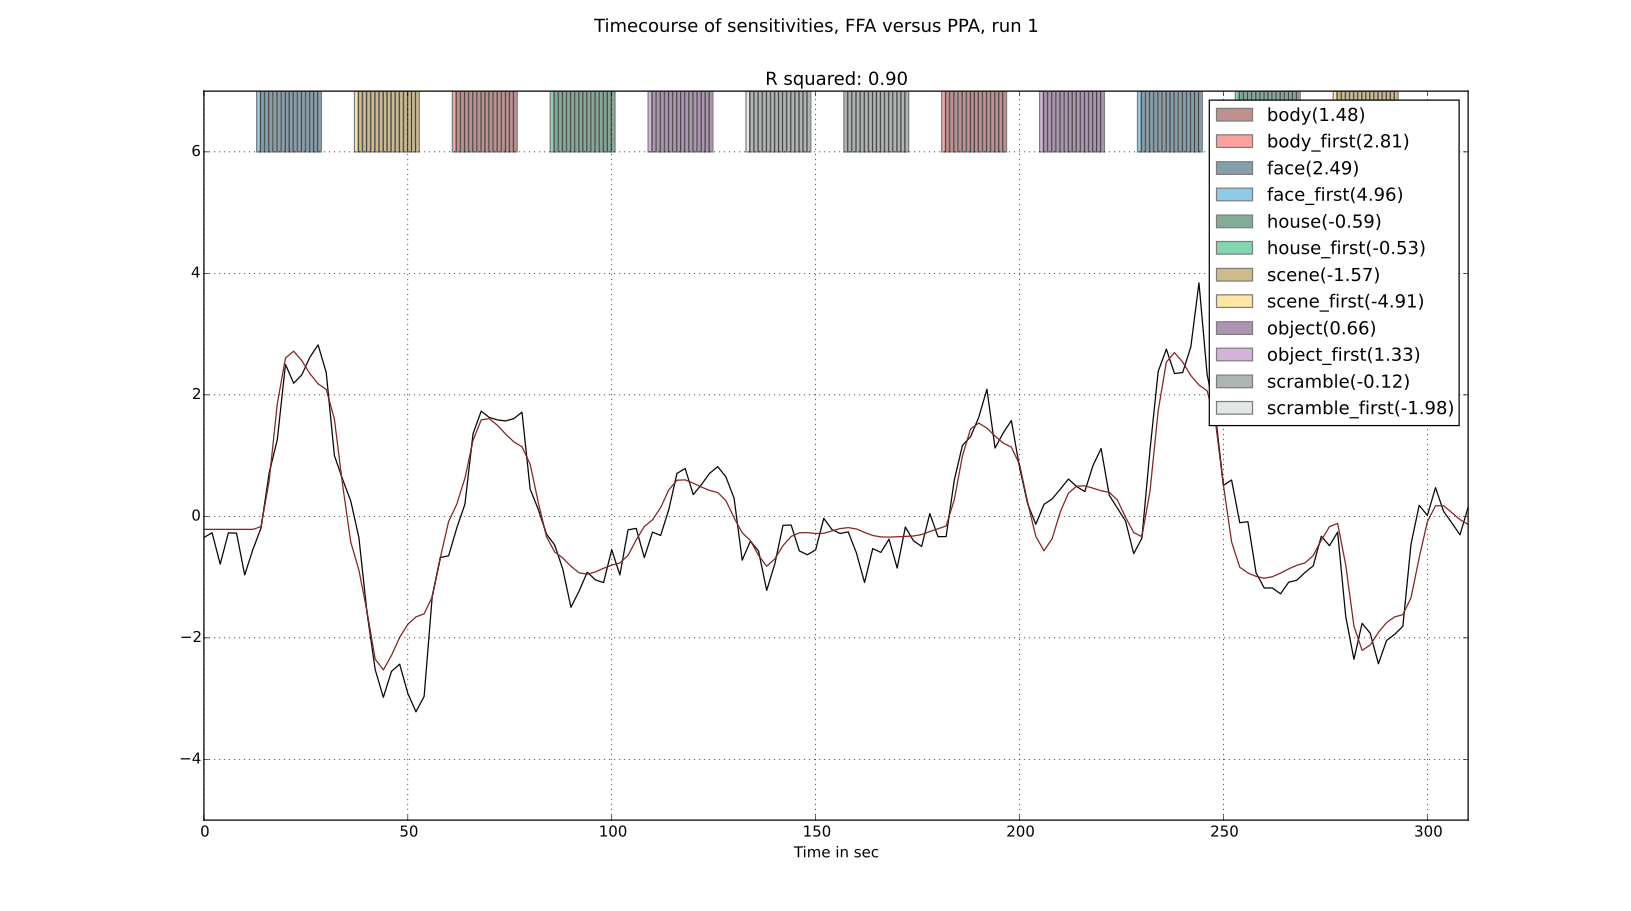
\includegraphics[scale=0.3]{img/tc_localizer.png}}
	\subfigure{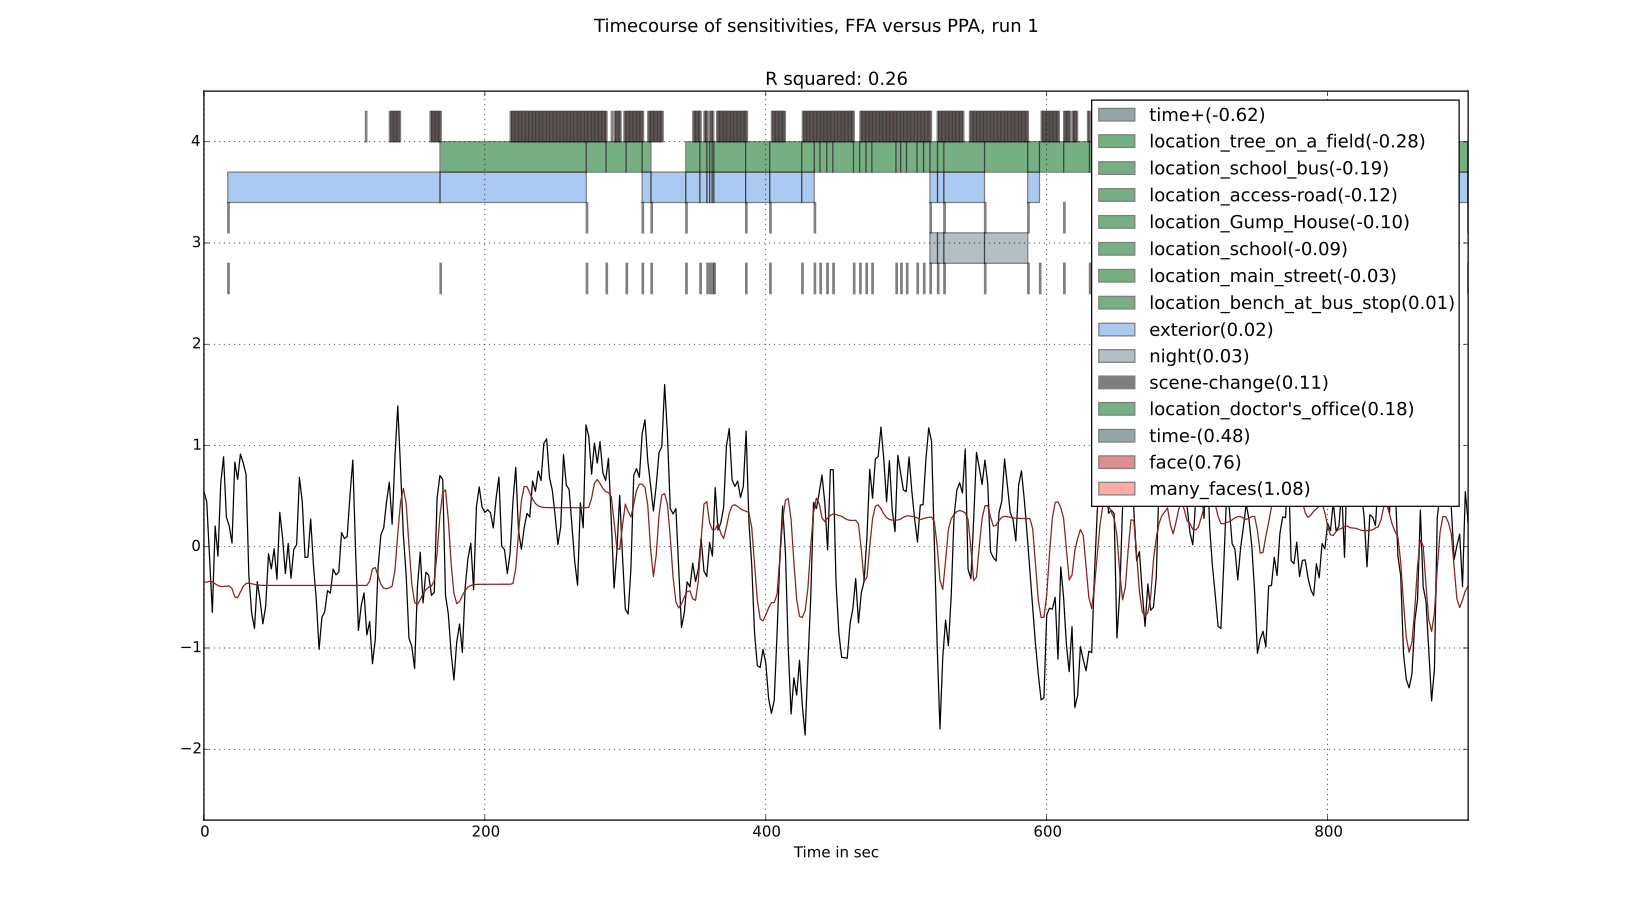
\includegraphics[scale=0.3]{img/tc_avmovie.png}}
	\caption[Functional specificity of ROIs in two proof-of-concept analyses.]{\small{Functional specificity of ROIs in two proof-of-concept analyses. Black line: Sensitivities. Red line: GLM fit from regressing sensitivities onto the event regressors. Top panel: Run 1 of the localizer experiment, with 12 regressors derived from the object categories of the stimulation. Bottom panel: Run 1 of the movie experiment with regressors derived from the movie annotation. The legend contains only those regressors that were present in the first run of the movie. Colors correspond to stimulation with one particular event type, beta values are given in brackets.}}
	\label{fig:locsens}
\end{figure}





\section{Discussion}\label{sec:c1_discussion}

This first chapter introduced a novel approach to determining functional specificity of regions of interest. To provide a proof-of-concept analysis, data from two different experiments conducted on the same participants was used to investigate the functional specificity of two well established ROIs, the FFA and the PPA. \newline
The results obtained during classification are of lesser interest for this thesis. However, they show some interesting results that I will briefly digress into. Importantly, as table \ref{tab:CV} summarizes, the GNB classifier performs comparable to the SGD classifier during classification. Despite the strong assumptions of the GNB algorithm, its classification hence appears to be robust. This provides a justification for further use of this classifier in the upcoming FEF investigation, which will benefit from the GNBs interpretable decision boundary parameters. Further, the table highlights very good and highly similar classification accuracies in both datasets. Note however that the higher accuracy in the full datasets may be misleading due an imbalance in class frequencies introduced by the inclusion of the 'rest of the brain': The higher accuracy stems from the high true positive rate of the rest of the brain voxels, which biases the overall accuracy. \newline 
Figure \ref{fig:CV} underlines the high accuracies and similarities in classification further: Both datasets show an almost perfect classification performance for FFA and early visual cortex, and good classification performance for LOC, FFA, and EBA. This finding shows that classification of ROIs is possible and highly accurate both with a standard block-design experiment and with dynamic, naturalistic stimulation. This replicates the findings of \textcite{nastase2016} and provides further evidence for the usability of complex, naturalistic stimulation for the localization of ROIs (\cite{malinen2007towards}).\\
The results obtained from the GLM provide a general proof-of-principle for the ROI specificity analysis. The validation analysis on the localizer paradigm shows a remarkable goodness of fit (R$^2$ = .90). The category information in the event files seems to be well able to capture the relative activation differences between the FFA and the PPA. The beta weights confirm known functional specificities of the ROIs, but they also reveal novel insights: As visible both from the time series' appearance and the regression coefficients, stimulation with images of faces ($\beta$ = 2.51) and, to a lesser extent, bodies ($\beta$ = 1.50), in particular the first of these stimuli per block ($\beta$=4.88 and $\beta$=2.78, respectively), differentially activated FFA more than PPA. The PPA in turn was differentially activated by stimulation with scenes (scene\_first: $\beta$ = -4.96, scene = $\beta$ = -1.59) and to a lesser extent houses (house\_first: $\beta$ = -0.53, house = $\beta$ = -0.59). The results therefore confirm that the FFA is differentially higher activated by pictures of faces, whereas the PPA is differentially higher activated by stimulation with houses (e.g. \cite{fox2009defining}). However, the results also show that, for one, the FFA is also activated by images of bodies, and the PPA is also activated by images of scenes. The most simple 'face-house' contrast may therefore not be the optimal choice of contrast. Additionally, the results reveal evidence for the influence of other stimulus features, such as the first image within a stimulation. Lastly, the results also contain data that does not correspond to results found in the literature: The first scrambled image contributes strongly to a differentially elevated PPA activation. There are several explanations for these findings. One may be that it is an artifact of random, high activation (outlier in the data), that has a strong influence on the beta weight due to the low amount of events in this regressor. However, this activation could also display mental processes associated with finding any recognizable pattern in this first scrambled image. Regardless of the explanation of this individual finding, summarizing this first glm, the analysis showed to work as intended for highly controlled experiments.
\newline
For complex, naturalistic stimulation in the movie experiment, the method proofed to be applicable as well. The lower goodness of fit indicates that the method provided only a partial explanation to the more complex sensitivity time course. Nevertheless, an R$^2$ of 0.26 still corresponds to a correlation of $r = .51$ between GLM fit and functional signature, and it is likely that additional annotations would improve the fit of the GLM. Additionally, the resulting regression coefficients are largely in line with previous results. The FFA is stronger activated than the PPA in the many\_faces ($\beta$=1.47) and face ($\beta$=1.04) conditions. These results show that an increase in the number of depicted faces in the movie also increases the relative activation of the FFA compared to the PPA. As displayed in figure \ref{fig:scenes}, locations consistently associated with higher FFA activation are more commonly depicting dialogues between two or more persons, whereas locations consistently associated with higher PPA activation are more commonly depicting urban or rural scenes. A finding that currently lacks a theoretical explanation is the association of temporal progression to the past or future with the FFA or PPA (regressors time+, time-).\\
Summarizing the results of both analyses, the method has provided evidence for its exploratory capabilities: In both analyses, it was able to give additional insights on the contribution of certain stimulus features to relative activation differences in the two exemplary ROIs. In this regard, the GNB classifier is a good choice of algorithm for the classification step, as it provides this straightforward interpretation of the time course of sensitivities, and yields robust results that are comparable in accuracy to the SGD with less strict assumptions. The method also showed to be applicable to confirming hypotheses testing. Even though not formally introduces as a hypothesis, the face annotation was included in the analysis as for the FFAs known functional specificities. The results confirm that the occurrence of faces corresponds to differentially higher FFA activation. Future analysis could use this capability to test hypotheses associated with specific annotated events. Even though both analyses used ROIs collapsed across hemispheres, a particularly interesting option this method offers is to analyze distinctiveness of ROIs between hemispheres. This approach will indeed be presented to investigate the research question set in this thesis and explore whether attention mode can distinguish left and right ROI from each other. Lastly, the method gives the possibility to analyze the functional specificity of one ROI compared to the rest of the brain (as this would be a valid second ROI for a pairwise comparison). \\ 
The affirmative results of the validation and generalization analysis warrant the subsequent use of this method for further steps in this Masters thesis. Using ROI masks obtained in chapter \ref{c2}, the ROI specificity method will be utilized in chapter \ref{c3} in an attempt to gain insights into hemispheric differences of the FEF with regard to attentional modulation. \\


\chapter{Localizing the frontal eye fields with naturalistic stimulation}\label{c2}

In the previous chapter, a novel approach to determining the functional specificity of ROIs was introduced and validated. To ultimately apply the method to explain a potential differential activation time course between the left and right FEF with attentional mode, ROI masks for this structure need to be derived. Therefore, this chapter describes the localization of the frontal eye fields, based on fMRI and eyetracking data obtained during movie watching. \\
In general, the approach for localization of the FEF follows the established patterns in functional ROI localization, a GLM contrasting the activation between a condition known to differentially activate the region in question, and a condition known to not activate the region in question. The complex, naturalistic stimulation of a Hollywood movie however requires an attempt at localization that relies on less experimentally controlled stimulation and unconstrained participant behavior. The potential benefits and caveats of this naturalistic stimulation in the localization of the FEF are outlined in section \ref{section:shortcomings}. \\ 
The involvement of the FEF in different movements of the eye, in particular its differential involvement in saccade generation (as section \ref{section:eyemoves} will describe), allows a contrast of saccade direction conditions that can be obtained from the eye tracking data recorded during movie watching. In order to derive said saccadic conditions, the raw eye tracking data were classified into different categories of eye movement by \textcite{dar2019}. A short overview of this is given in section \ref{c2:remodnav}. Afterwards, section \ref{c2:fitlins} will outline the selection of a contrast of choice and its implementation in the software \texttt{fitlins} for automatic GLM fitting of data in BIDS (\cite{gorgolewski2016brain}) or BIDS-Derivatives compliant datasets. Section \ref{c2:masks} discusses the final mask creation based on the GLM results.


\section{Insights on FEF location from naturalistic stimulation}\label{section:shortcomings}
Localization of areas involved in motor tasks such as the FEF is most reliably conducted via micro-stimulation with small electrical currents applied directly to populations of neurons (see eg. \cite{bruce1985primate}). However, such approaches are only rarely possible in human subjects. Localization through non-invasive methods is more challenging, yet it is a necessary prerequisite for further research about the FEF. Paradigms for the localization of the FEF usually employ simple behavioral tasks with either general (\cite{paus1996location}), or specific oculomotor movements such as instructed fixations, pro- and antisaccades (\cite{connolly2002human}), or tracking of horizontal step stimuli (\cite{alkan2011differentiation}). These paradigms bear the advantages of highly controlled, predictable participant behavior, and enforcement of all possible saccadic target positions, onset positions, and amplitudes. However, while capable of localizing areas undoubtedly involved in the movement of the eyes, the displayed movements are not performed under unconstrained conditions. For regions involved in higher cognition such as the FEF it remains unknown whether uncontrolled eye movements under naturalistic viewing behavior can be capable of providing similar, if not even additional information. Previous localization studies employing positron emission tomography (PET) (e.g. \textcite{paus1996location}, \cite{kawashima1998oculomotor}), magneto-encephalography (MEG) (e.g. \cite{ioannides2004meg}), fMRI (e.g. \cite{petit1999functional}; \cite{connolly2002human}), and transcranial magnetic stimulation (TMS) (see \textcite{vernet2014corrigendum}, for an overview) were able to shed light on the possible location of the FEF in humans. However, an overall view of this literature also reveals the large variability of reported localizations between studies (see e.g. \textcite{paus1996location}; \textcite{vernet2014corrigendum}, for overviews), and there is no consensus on whether these discrepancies arise from methodological differences in the choice of imaging technique or behavioral paradigm, or inter-individual differences between participants. A more naturalistic paradigm might be able to provide additional answers to this question. \newline
In order to localize the FEF of the studyforrest participants, and attempt a classification with unconstrained gaze that additionally may address the blank spaces left by paradigms with highly controlled, simplistic stimuli or tasks, this chapter presents the use of a more ecologically valid stimulation paradigm by using fMRI and eye-tracking data obtained during movie watching. 



\section{Movements of the eye}\label{section:eyemoves}

\textbf{A bit of an introduction here, please....}\\ A central feature of the human eye is the fovea centralis, a specialised region about 1.5mm in diameter in the center of the retina (\cite{benninghof2004anat}). It serves only the central 1$^\circ$ of the visual field, but due to possessing the highest amount of cones of the retina, and an asymmetric distribution of ganglion cell density across the retina that advantages foveal information, it provides the greatest visual acuity (\cite{perry1986ganglion}). This asymmetry is propagated in the cortical representation of visual inputs from the retina. The magnification factor (MF), the linear extent of cortex devoted to each linear degree on the retina, increases monotonically from periphal to foveal vision (\cite{daniel1961representation}). As a result, in almost all visual brain areas, both cortically and subcortically, the fovea has the greatest representation, and full visual acuity can hence only occur at the fovea. Due to this constraint, humans need the ability to, first, align the fovea rapidly to an object of interest in a visual scene and, second, keep the fovea aligned to it for a sufficient amount of time in order to maximize the efficiency of foveal vision and perceive objects of interest in greatest detail. An exploration of a visual scene is hence performed in a stepwise manner and requires the described sequence of eye movements to sequentially explore all areas of interest. To accomplish this, the human eye is capable of a number of different eye movements. In its most simple form, the sequence consists of rapid saccadic eye-movements, redirecting the fovea from one object of interest to the next, followed by phases of fixation that keep the fovea aligned for visual analysis. Unconstrained vision as during movie watching will therefore require continuous eye movements to view content depicted at different parts of the screen with highest visual acuity.\newline
As outlined in the section \ref{section:visualattention}, the FEF are involved in almost all types of eye movements, but specifically saccadic eyemovements (\cite{leichnetz1988higher}). The FEF does not control all saccades, though. Interestingly, early stimulation studies showed a distinction between horizontal and vertical saccades. The frontal eye fields are involved in the generation of saccades to the contralateral space in horizontal, oblique up or oblique down directions in the visual field (see \textcite{bruce1985primate}, \textcite{blanke2003direction}). Activation of the right FEF leads to conjugate eye movement to the left, and vice versa. Vertical saccades, however, are utilizing different neuronal circuitry distributed diffusely around the cortex, that ultimately project into the rostral interstitial nucleus of the medial longitufinal fasiculus (riMLF) and the interstitial nucleus of Cajal in the mesencephalon (\cite{FUKUSHIMA1991159}). These different underlying neural circuitry for horizontal and vertical eye movements can be observed in human stimulation studies (\cite{blanke2003direction}), but also in neurodegenerative diseases that affect those oculomotor nuclei involved in vertical saccades: Supranuclear palsy (PSP) and pure akinesia (PA) (\cite{rottach1996dynamic}, \cite{riley1994syndrome}), or midbrain lesions (\cite{ranalli1988palsy}) lead to differential impairment of vertical but not horizontal eye movement. Regarding stimulation studies of the FEF, only a few studies reported to evoke purely vertical saccadic eye movements, and \textcite{blanke2003direction} concluded that "all human studies agreed that electrically induced EM [eye movements] are mainly contralateral as well as horizontal". In their own electrical stimulation study in five epilepsy patients, \textcite{blanke2003direction} found $66\%$ of all evoked saccades to be along the horizontal meridian, $34\%$ to be oblique upward or downward, and no saccade to be purely horizontal or vertical. Non-invasive localization paradigms of the FEF mirror these findings and often use saccadic targets along the horizontal meridian (\cite{connolly2002human}; \cite{alkan2011differentiation}).
Based on this theoretical reasoning, a contrast between activation during horizontal and vertical saccadic eyemovements made by participants during movie watching is used to localize the frontal eye fields.


\section{Methods}
The envisioned localization analysis required some additional software. For a classification of raw eye tracking data into categories of eye movements, the analysis relied on results obtained with a novel eye movement classification algorithm (section \ref{c2:remodnav}). The actual localization was performed with fitlins (\cite{markiewicz_christopher_j_2019_2555453}) and required additional software implementations and restructuring of dataset repositories (see section \ref{c2:fitlins}).

\subsection{Analysis-specific data}
The localization of the FEF uses the custom preprocessed BOLD data from the movie experiment (see section \ref{section:generalmethods}) together with the eye tracking data that were obtained simultaneously. 
In addition, several confounds were included in the analysis: For one, the motion parameters derived during motion correction and distributed along in the studyforrest publication as mcparams.txt files. Secondly, unpublished stimulus confounds consisting of computations of the framewise root mean square power (RMS) of the audio track, the left-right difference of the RMS (lrdiff), and the perceptual difference between frames (pd). The latter confounds were used to explain potential variance in BOLD data introduced by stimulus features irrelevant for the current research question. All code for this analysis can be found on Github\footnote{https://github.com/AdinaWagner/BIDSsacc}.


\subsection{Classification of eye events with REMoDNaV}\label{c2:remodnav}

In order to extract all saccadic eyemovements, the eye-tracking data was classified into different eye movements. For this, based on an adaptive, velocity-based algorithm proposed by \textcite{nystrom2010adaptive}, \textcite{dar2019} implemented a data-driven algorithm for robust eye movement detection for natural viewing (REMoDNaV) in Python\footnote{The sourcecode can be found at github.com/psychoinformatics-de/remodnav. All results of this algorithm will be made publicly available after publication at https://github.com/psychoinformatics-de/studyforrest-data-eyemovementlabels}. The algorithm categorizes the raw data into the eye movement categories saccades, fixations, smooth pursuits and post-saccadic oscillations, and disregards any unclassifiable data (such as blinks). The eye events are reported together with their start- and end coordinates, their onsets and duration in seconds, their velocity and the average pupil size.

\subsection{FEF localization with saccadic eye movements and fitlins}\label{c2:fitlins}
Subject-specific localization of the frontal eye fields is performed based on each subjects saccadic eye movements throughout the movie. For the extraction of saccadic eye events, the REMoDNaV results were filtered to include only saccades. For the computation of event files following the BIDS standard (\cite{gorgolewski2016brain}), the Cartesian coordinates of the saccades were transformed into Polar coordinates (angle and length, a graphic explanation of this procedure can be found in figure \ref{fig:Polar_to_cartesian}, B). Based on their angle, saccades were classed into event types describing 12 different orientations in the visual field. Four of these quadrants corresponding to 30$^\circ$ around the horizontal and vertical axis (see figure \ref{fig:saccs}) were sub-selected to be used for localization, and the saccades onsets, durations and amplitudes were extracted from the REMoDNaV output. The resulting event file per run hence contained the columns onset, duration, amplitude and trial\_type (containing four saccade directions as strings 'UP', 'DOWN', 'LEFT', 'RIGHT').

\begin{figure}[H]
	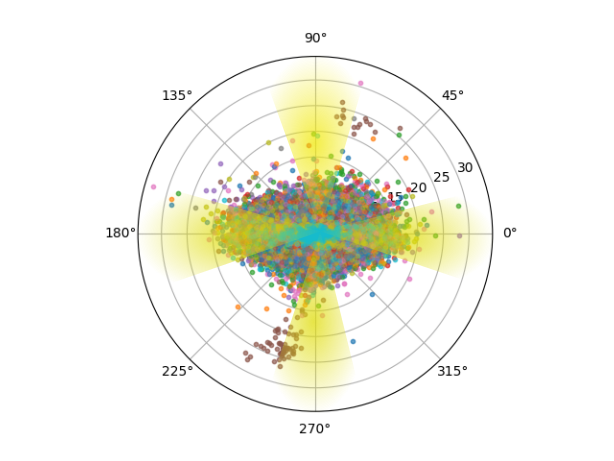
\includegraphics[scale = 0.7]{img/saccades.png}
	\caption[saccadic eye movements during movie watching]{\begin{small}Polar coordinates (direction in degrees on the outer ring, length in visual degrees on the inner grid) of saccadic eyemovements of all subjects during movie watching. Colors indicate subjects. Yellow overlay indicates 30$^\circ$ around the horizontal or vertical axis.\end{small}}
	\label{fig:saccs}
\end{figure}

All four directions were entered as regressors into a fixed-effects three-level GLM\footnote{Note that in theory, a two level (run, subject) GLM would have sufficed - fitlins however does not yet contain functionality to subselect analysis levels. Fitlins also does not yet contain functionality to perform mixed- or random effects modeling.} (run, subject, dataset) to localize the FEF. GLM computation was done with fitlins (\cite{markiewicz_christopher_j_2019_2555453}). Fitlins is a software for estimating linear models on BIDS or BIDS-derivatives (\cite{gorgolewski2016brain}) compliant data directories. It relies heavily on pybids (\cite{yarkoni_tal_2019_2555449}) to automatically query and ingest all relevant data files, and is intended to be run with only one commandline call. As a first step, therefore, the directory was restructured to be BIDS-derivative compliant, motion parameter .txt files were transformed into dense \_regressors.tsv files, and confounds relating to the movie stimulus were transformed into one dense \_physio.tsv.gz file.
Figure \ref{fig:dirstruct} gives an overview of the directory structure for one subjects and one run. To compute a linear model with fitlins, a model\_smdl.json file specifies the desired analysis-levels, regressors and their transformations, and contrasts. For the localizer GLM, fitlins \texttt{Split} transformation was used to obtain four saccade direction regressors with their amplitude, and the \texttt{Convolve} transformation was used to convolve all regressors with spm's HRF function. The full model\_smdl.json file used for the localizer GLM can be found in appendix \ref{A:fitlins}. The weights $[1, 1, -1, -1]$ for regressors 'LEFT', 'RIGHT', 'UP', 'DOWN' are used to define a horizontal-vs-vertical eye movements contrast, and this contrast is carried through all higher levels with fitlins \texttt{AutoContrasts} functionality. \newline

\begin{figure}
	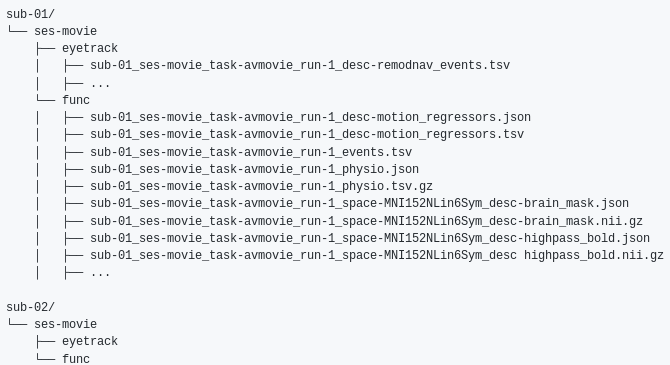
\includegraphics[scale=0.7]{img/dirstruct.png}[H!]
	\caption[BIDS derivatives directory structure]{\begin{small}The BIDS derivatives conform directory structure of the dataset, shown here for subject 1, run 1.\end{small}}
	\label{fig:dirstruct}
\end{figure}

As fitlins is still in early alpha stage development phase, as it had never been used on a sole BIDS derivatives directory, as the inclusion of eye-tracking data is not yet integrated into the BIDS standard\footnote{There is however work in progress on a BIDS Extension Proposal 20 (BEP020), that this thesis relied upon.}, and as the employed design was more complex than a regular block-stimulation experiment, the implementation of the model led to multiple failures on every stage of the analysis. In the wake of model implementation, several contributions have therefore been made to the recent releases of fitlins (\cite{markiewicz_christopher_j_2019_2555453}) and pybids (\cite{yarkoni_tal_2019_2555449}), leading to a co-authorship in both of these software's releases.
Despite these improvements, the current model relies on some custom source code changes not (yet) integrated into the main software distribution. In order to recreate the computational environment necessary for reproducing the analysis, a niceman.yml\footnote{Niceman (very recently renamed to 'Reproman') (\cite{yaroslav_halchenko_2018_2403222}) is a software that analyzes and summarizes computational environments for later recreation and recomputation: https://github.com/ReproNim/reproman} file is part of the directory. 

\subsection{Creation of ROI masks}\label{c2:masks}
In order to obtain subject-specific ROI masks, an attempt was made to find clusters corresponding to the FEF in the subject-level result of each participant with FSLeyes (\cite{mccarthy_paul_2018_1887737}). Mimicking \textcite{sengupta2016studyforrest}, a cluster-forming threshold of z = 1.64 was used. Clusters were selected based on the known anatomical location of the FEF, and Neurosynths (\cite{yarkoni2011neurosynth}) posterior probabilities of relevance of corresponding terms to brain locations\footnote{Neurosynth was used with the fsl-neurosynth-atlas as distributed in the NeuroDebian (\cite{10.3389/fninf.2012.00022}) platform}. Clusters surviving the thresholding at a plausible location were hand-traced into binary ROI masks. \\
As table \ref{tab:masks} shows, however, this approach was unable to identify masks for 10 out of the 30 masks. For remainder of FEFs, a grouplevel mask obtained from the result of the dataset-level with the same procedure was substituted.

\section{Results}

In order to check the validity of the eye-movement extraction with REMoDNaV, the mean and median duration of extracted fixations were compared to the results of \textcite{dorr2010variability}, who studied descriptive parameters of eye movements during movie watching. Fixations as found by REMoDNaV had a length of mean = 0.326s, median = 0.256s, which corresponds closely to the aforementioned study's results (0.354s and 0.253s, respectively). A comparison of algorithm performance and human coding of eye movements on data of \textcite{andersson2017one} by \textcite{dar2019} found that REMoDNaV had the highest degree of concordance of all contemporary algorithms used in \textcite{anderson2015comparison}, providing further evidence for the validity of extracted eye movements. \newline
\textbf{TODO: summary stats about saccade directions and amplitudes, maybe a bar plot.}

\begin{figure}[h]
	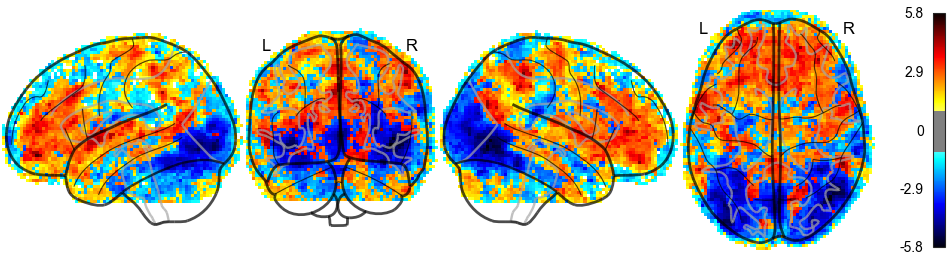
\includegraphics[scale=0.6]{img/3rdlvl_fitlins.png}
	\caption[GLM results with fitlins]{\small{Glass brain plot of the third-level results for the horizontal-vs-vertical contrast.}}
	\label{fig:fitlins}
\end{figure}

Figure \ref{fig:fitlins} shows a glass brain plot of the third-level GLM results. Out of the 15 subjects, 12 subject-specific masks for the right FEF and, 8 subject-specific masks for the left FEF were obtained from the second-level GLM results. Table \ref{tab:masks} summarizes minimum and maximum coordinates as well as the location with the highest activation of obtained masks per participant and hemisphere. Figure \ref{fig:FEF} displays the overlap of the resulting FEF masks.

\begin{figure}[H]
	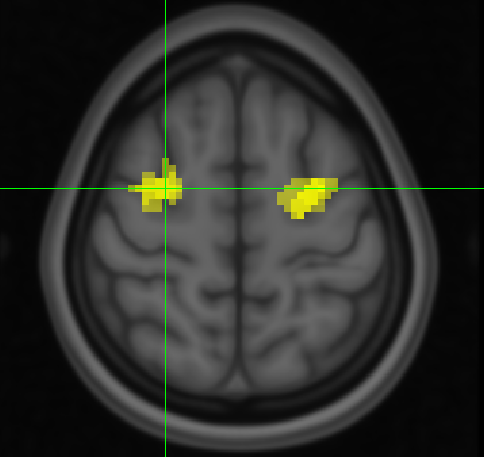
\includegraphics[scale=0.35]{img/FEF_masks_overlaid_v2.png}
	\caption[]{\small{Subject-specific ROI masks overlaid on a group-space template (screenshot of the FSLeyes interface). Regions with lower opacity correspond to higher overlap of masks.}}
	\label{fig:FEF}
\end{figure}

\begin{table}[H]
	\centering
	{\scriptsize
	\begin{tabular}{C{1.5cm}C{1.2cm}C{1.2cm}C{1.2cm}C{1.2cm}C{1.2cm}C{1.2cm}C{3cm}}
		\thickhline
		\textbf{right} \\
		\thickhline 
		\textbf{subject}	& \textbf{min x} & \textbf{min y} & \textbf{min z} & \textbf{max x} & \textbf{max y} & \textbf{max z} & \textbf{max activation}  \\ \hline
		1	& $60$    & $4$ & $50$ & $37$ & $-5$ & $42$ & $(42, -3, 48)$\\
		2	& $-$   & $-$ & $-$ & $-$ & $-$ & $-$ & $-$ \\			
		3	& $42$    & $3$ & $46$ & $31$ & $-4$ & $41$ & $(38, 4, 41)$\\			
		4 & $30$  & $2$ & $46$ & $31$ & $-4$ & $41$ & $(25, -3, 51)$ \\
		5	& $-$   & $-$ & $-$ & $-$ & $-$ & $-$ & $-$ \\
		6	& $43$   & $5$ & $50$ & $27$ & $-6$ & $40$ & $(28, 1, 45)$ \\ 
		9	& $-$   & $-$ & $-$ & $-$ & $-$ & $-$ & $-$ \\
		10	& $37$   & $2$ & $58$ & $22$ & $-10$ & $43$ & $(33, -5, 48)$ \\
		14	& $42$   & $4$ & $43$ & $22$ & $-5$ & $40$ & $(32, -1, 48)$ \\
		15	& $48$   & $7$ & $48$ & $28$ & $3$ & $43$ & $(38, 5, 46)$ \\
		16	& $40$   & $2$ & $61$ & $25$ & $-8$ & $43$ & $(40, -2, 56)$ \\
		17	& $40$   & $5$ & $53$ & $26$ & $-3$ & $53$ & $(29, -2, 46)$ \\
		18	& $43$   & $-1$ & $48$ & $40$ & $-9$ & $43$ & $(43, -7, 46)$ \\
		19	& $50$   & $4$ & $50$ & $37$ & $-5$ & $42$ & $(42, -3, 48)$ \\
		20	& $30$   & $7$ & $58$ & $24$ & $-3$ & $53$ & $(28, 2, 58)$ \\
		mean & & & & & & & $(34 \pm 6, -1 \pm 3, 48 \pm 5)$\\\thickhline
		\textbf{left} &&&&&&&\\\thickhline
		1	& $-38$    & $0$ & $57$ & $-25$ & $-10$ & $50$ & $(-31, -6, 52)$\\
		2	& $-$   & $-$ & $-$ & $-$ & $-$ & $-$ & $-$ \\			
		3	& $-38$    & $5$ & $46$ & $-21$ & $-3$ & $41$ & $(-30, 3, 43)$\\			
		4 	& $-$   & $-$ & $-$ & $-$ & $-$ & $-$ & $-$ \\ 
		5	& $-$   & $-$ & $-$ & $-$ & $-$ & $-$ & $-$ \\
		6	& $-40$   & $3$ & $50$ & $-26$ & $1$ & $43$ & $-$ \\ 
		9	& $-$   & $-$ & $-$ & $-$ & $-$ & $-$ & $-$ \\
		10	& $-30$   & $-3$ & $58$ & $-16$ & $-9$ & $56$ & $(-25, -4, 58)$ \\
		14	& $-$   & $-$ & $-$ & $-$ & $-$ & $-$ & $-$ \\
		15	& $-$   & $-$ & $-$ & $-$ & $-$ & $-$ & $-$ \\
		16	& $-42$   & $-1$ & $60$ & $-22$ & $-12$ & $48$ & $(-21, -8, 55)$ \\
		17	& $-50$   & $-1$ & $55$ & $-24$ & $-13$ & $43$ & $(-33, -8, 48)$ \\
		18	& $-$   & $-$ & $-$ & $-$ & $-$ & $-$ & $-$ \\
		19	& $-48$   & $1$ & $55$ & $-39$ & $-8$ & $43$ & $(-48, -5, 53)$ \\
		20	& $-40$   & $1$ & $58$ & $-29$ & $-4$ & $53$ & $(-38, 1, 55)$ \\
		mean & & & & & & & $(-32 \pm 8, -4 \pm 4, 52 \pm 5)$\\\thickhline
		\caption[FEF masks coordinates]{\small{Minimum and maximum coordinates of the subject-specific FEF masks, and the voxel location with the highest activation, for left and right FEF.}}
		\label{tab:masks}
	\end{tabular}}
\end{table}


\section{Discussion}

As evident from table \ref{tab:masks}, the location of the derived FEF masks varies between subjects. In general, however, the obtained coordinates lie in Brodmans Area 6, which corresponds to human fMRI studies (\cite{vernet2014corrigendum}), and the average activation maxima correspond to probable FEF locations found by others as well (e.g. \cite{paus1996location}; \cite{tehovnik2000eye}; Luna et al. (1998), cited by \textcite{vernet2014corrigendum}). The large range in individual x-coordinates suggests that activation in both the ventrolateral region, generating shorter saccades (2-15$^\circ$, \cite{bruce1985primate}), and mediodorsal region, generating longer saccades (13-25$^\circ$, \cite{bruce1985primate}), has been captured by the contrast. This is in accordance to figure \ref{fig:saccs}, which shows that saccades of up to 30$^\circ$ we evoked by the movie stimulus. \\
However, the analysis failed to find activation clusters in ten cases. This can be partially attributed to subjects with high data loss (e.g. subject 5 with 85\% of the eye tracking data containing no signal). Another contributing factor might be that purely vertical saccades occur less frequent than horizontal saccades, and short saccades are much more frequent than longer saccades (see \ref{fig:saccs}). As such, the movie stimulus may not be an optimal stimulus choice: The gaze of participants might be too centered to evoke the necessary activation. Studies into the distribution of gaze during different visual stimuli find that such a center bias occurs in particular within Hollywood movies (see e.g. \cite{tseng2009quantifying}). \\ Additionally, the sluggish nature of the fMRI signal likely hinders efforts to accurately pinpoint saccadic events in time. The high temporal resolution of the eye tracker with a sampling rate of 1000Hz can not be propagated to the BOLD signal. The unconstrained eye movements of participants additionally mix all possible types of eye movements. Therefore, unlike eye movement block design paradigms that control for blinks or fixations and saccade  direction, the vast amount of intermixed eye movements could constitute a problem for the localization. It is further notable that the right FEF was located more frequently than the left FEF, even though there is no evident bias to the left hemifield in saccade distribution. This may reflect a right hemispheric dominance as found in other studies \textbf{cite something}. \\
Nevertheless, this localization with eye tracking data from naturalistic stimulation did succeed for two thirds of all cases and on the group level, and the coordinates of the resulting ROI masks appear to be in accordance to the results of other non-invasive neuroimaging studies. These findings, at least in part, provide further evidence for the use of naturalistic stimulation in favor of standard paradigms, however, Hollywood movies with their strong center bias are not an optimal stimulus choice. More natural scenes, for example undirected and unprocessed recordings of everyday scenes such as in \textcite{tseng2009quantifying} could evoke larger and more distributed saccadic eye movements. The obtained FEF masks are used in the next steps to include an FEF ROI into the functional specificity analysis.



\section{Discussion}
\textbf{TODO: Do a discussion here}
include:
\begin{itemize}

	\item{discuss shortcomings of fitlins}
	
\end{itemize}


\chapter{The functional specificities of the Frontal Eye Fields}\label{c3}

The previous chapters described the implementation and validation of a novel method to determine functional specificity of ROIs, and the computation of a GLM with fitlins to localize the frontal eye fields. The following chapter will combine the efforts of these sections with a measure of attentional mode during movie watching to investigate the main research question of this thesis.\\
As a first step, the eye gaze data of participants was used to compute a measure of attentional mode exerted by the movie stimulus. For this, a multidimensional scanpath comparison algorithm was ported into a Python module, adapted to the peculiarities of a movie stimulus, and used to compute the similarity of temporo-spatial eye gaze sequences of all subjects per shot. Section \ref{section:eyeutils} discusses the reasoning behind an attentional mode measure from eyegaze, while section \ref{section:multimatch} elaborates on the algorithm and its dataset specific adaptations.
In a final step, the obtained FEF masks from chapter \ref{c2} were included into the movie group-dataset used in chapter \ref{c1}, and the derived similarity dimensions of section \ref{section:multimatch_attention} were entered as regressors in a GLM to investigate whether the attentional mode could explain potential activation differences of the left and right FEF (see section \ref{c3:FEF}). 

\section{Utilizing eye movements in the study of attentional deployment}\label{section:eyeutils}

In order to include the aspect of visuospatial attention mode, a quantitative measure of attentional deployment needs to be derived. One possibility to do this is by using eye gaze information in the form of \textit{scanpaths}.
The term scanpath refers to the trace of eye-movements in space and time (\cite{holmqvist2011eye}). In its most simple form, it is formed by a succession of fixations and saccades that define the particular sequence in which the eyes explore a visual scene (\cite{anderson2015comparison}). As opposed to other measures that summarize eye gaze, such as heatmaps, the order of eye-movements is relevant - a different order of elements in the representational sequence of eye-movements constitutes a different scanpath. \newline
The analysis of scanpaths has been used for decades to gain insights into the viewers’ mental processes, especially those concerning visuo-spatial attention. \textcite{yarbus1967eye} wrote: 

\begin{quotation}
\footnotesize{„Eye-movements reflect the human thought processes; so the observer‘s thoughts may be followed to some extent from records of eye-movements (the thought accompanying the examination of the particular object). It is easy to determine from these records which elements attract the observer‘s eye (and, consequently, his thought), in what order, and how often.“}
\end{quotation}

Following this reasoning, the comparison of scanpaths of different subjects constitutes a measure of similarity in the different subjects’ attentional processes and adds a useful dimension to the traditional analysis of eye-tracking data. \newline
In recent years, many approaches for scanpath comparisons were developed and implemented in various software solutions. Among them are methods based on (semantic) areas of interest (AOIs) such as the \textit{Levenshtein distance} (\cite{levenshtein1966binary}), or an improved generalization of it in \textit{ScanMatch} (\cite{cristino2010scanmatch}), methods based on attention maps such as \textit{AMAP} (\cite{ouerhani2004empirical}), methods employing machine learning algorithms such as \textit{SMAC with HMM} (\cite{coutrot2018scanpath}), or methods based on vector-geometry such as \textit{MultiMatch} (\cite{jarodzka2010vector}). The latter method is a multidimensional approach of scanpath comparison on five different measures similarity, \textbf{shape}, \textbf{length}, \textbf{position}, \textbf{direction}, and \textbf{fixation durations}. According to \textcite{jarodzka2010vector}, it has been developed specifically to overcome known shortcomings of many previous methods that limit their informative value. These shortcomings amount to a loss of information due to the use of coarse aggregate measures of eye movement, susceptibility of the results of a comparison to influential data points due to arbitrary classifications, or both. The main reason it overcomes these deficiencies is that it does not rely on AOIs, but the precise locations in pixels in two-dimensional space, which leads to a finer level of detail in scanpath comparison. \newline A number of studies used the method in evaluations or applications of scanpath comparisons. In evaluations with simulated and actual eye-tracking data, the method was found to be robust against spatial noise, sensitive to position, order and fixation duration, and outperformed the ScanMatch method in AOI border cases (\cite{dewhurst2012depends}). In a comprehensive test of eleven common scanpath comparison methods on static real-life photographies, MultiMatch was found to be robust in inter- and intra-subject comparisons of scanpaths (\cite{anderson2015comparison}). As it was also used to study mental activity involved in perceiving visual input by others (\cite{french2017evaluation}) already, the MultiMatch algortihm was employed in the current thesis to derive a measure for attentional processes of participants during movie watching. \newline
For its computation, this attentional measure utilizes the scanpath information of all participants to obtain a common measure of attentional modulation of the stimulus in the sample. It follows a reasoning conceived by \textcite{baumgartner}: The more similar all participants scanpaths are for any given scene of a movie stimulus, the more exogenous control is exercised by this movie segment. Less exogenous control, i.e. lower scanpath similarity, would in turn correspond to a more endogenous attention mode. In a study of the contribution of visual features in dynamic scenes to gaze clustering, \textcite{mital2011} followed the same thought, and summarized it like this:
\begin{quotation}
	Being involuntary, exogenous control
	should be consistent across all viewers leading to a high
	degree of coordination in where and when multiple viewers
	attend given the same stimuli. By comparison, endogenous
	control should result in less coordination of attention across
	individuals as the internal cognitive states of the individual
	and their relation to the current stimuli are less predictable.
\end{quotation}.
A comprehensive overview of the method and the attention mode measure is given the following sections.
 
\section{Methods}
The first part of this section is dedicated to the MultiMatch algorithm. The second part elaborates on the application of the ROI specificity analysis for the study of the frontal eye fields.
\textbf{more more more more more...}
\subsection{Analysis-specific data}

This analysis uses the custom preprocessed BOLD files from the movie experiment (see section \ref{section:generalmethods}), the eye tracking classification by REMoDNaV (see section \ref{c2:remodnav}), the FEF ROI masks derived in the chapter \ref{c2}, and the annotation confounds by \textcite{hausler2016annotation}.

\subsection{MultiMatch}\label{section:multimatch}

The MultiMatch method (\cite{jarodzka2010vector}) is a promising approach of scanpath comparison. The original implementation, however, only existed as a Matlab toolbox shared upon request by the corresponding author of the respective publication (\cite{dewhurst2012depends}). This reliance on closed-source software and barriers in retrieval of the software\footnote{While acquisition of the toolbox via e-mail was prompt and complication-free, later correspondence with several of the authors was an odyssey of expired email addresses, changed affiliations and digital communication allegedly lost in the void of the Internet.} hinder the wider usage and potential improvement of the method. A publicly available, open-source implementation would instead facilitate its usage in scientific works. Therefore, the method was ported from Matlab into Python and transformed into the pip-installable module \textit{multimatch}\footnote{The module can be installed via ``pip install multimatch``. A corresponding publication (Wagner \& Hanke) in the Journal of Open Source Software (JOSS) in currently in preparation. The sourcecode can be found at github.com/AdinaWagner/multimatch.}.

\subsubsection{multimatch in Python}
The following section gives a brief overview of the general MultiMatch method. An overview in pseudocode is outlined in algorithm \ref{algo:multimatch}. \newline 
The method takes two n x 3 fixation vectors of two scanpaths with x-coordinates in pixel, y-coordinates in pixel, and duration of fixations as columns as its input. Based on the coordinates and durations of fixations, the scanpaths are represented as geometric vector sequences as shown in figure \ref{fig:Polar_to_cartesian}:

\begin{figure}[H]
	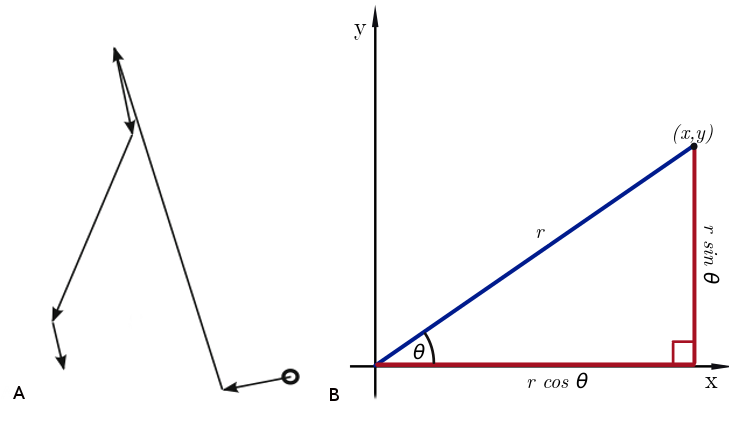
\includegraphics[scale=0.35]{img/scanpathconversion.png}
	\caption[Geometric representation of eye movements]
	{\small{\textit{A: Geometric scanpath representation.} An idealized saccade is represented as the shortest distance between two fixations. The Cartesian coordinates (x, y) of the fixations are thus the starting and ending points of a saccade. The length of a saccade in x (or y) direction is computed as the difference in x (or y) coordinates of starting and ending point. \newline
			\textit{B: Length and angle computation.} Length from the coordinate origin, rho, is computed as the Euclidean norm by means of the Pythagorean theorem: $r = \sqrt{ x^2 + y^2}$. The angle in radians, theta, is computed as a variation of the arctangent function as the angle from positive x axis to the point (x, y), with positive values denoting counterclockwise angle from positive x axis and negative values denoting clockwise angles: $\theta = arctan2(x, y)$.}}
	\label{fig:Polar_to_cartesian}
\end{figure}

To reduce complexity, the scanpaths are simplified according to angle and amplitude in an iterative procedure. Two or more saccades are grouped together if angles between two consecutive saccades are below an angular threshold \textit{TDir}, or if the amplitude of successive saccades is below a length threshold \textit{TAmp}, as long as intermediate fixations of the saccades are shorter than a duration threshold, \textit{TDur}. As such, small, locally contained saccades, and saccades in the same general direction are summed to form larger, less complex saccades. \newline
In order to find pairings of saccade vectors to compare, the simplified scanpaths are temporally aligned. The aim is to not necessarily align two saccade vectors that constitute the same component in  their respective vector sequence, but those two vectors that are the most similar while still preserving temporal order. In this way, a stray saccade in one of the two scanpaths does not lead to an overall low similarity rating, and it is further possible to compare scanpaths of unequal length.  To do so, all possible pairings of saccades are evaluated in similarity by the vector differences between all pairings (shape): The vector differences between each element $i$ in scanpath $S1 = {u_1, u_2, \ldots, u_m}$ and each element $j$ in scanpath $S2 = {v_1, v_2, \ldots, v_n}$ are computed and stored in a matrix $M$ with dimension m x n as weights that denote similarity, with low weights corresponding to high similarity. In a next step, an adjacency matrix is build, defining the rules on which connection between matrix elements are allowed to preserve the temporal order of saccades: In order to take temporal sequence of saccades into account, connections can only be made to the right, below or below-right (green arrows in figure \ref{fig:directedgraph}). Together, matrices $M$ and the adjacency matrix constitute a matrix representation of a directed, weighted graph (figure \ref{fig:directedgraph}). Elements of the matrix are nodes, the connection rules constitute edges and the weights define the cost associated with each connection. 
In the generic example in figure \ref{fig:directedgraph} the edge between node (1, 1) and node (1, 2) has an associated weight, or cost, of $w_2$. 


\begin{figure}
	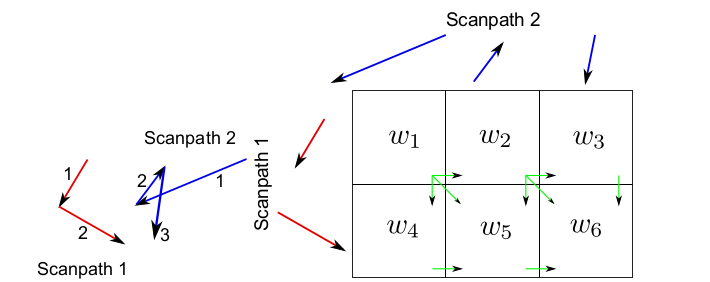
\includegraphics[scale=0.4]{img/weightedgraph.png}
	\caption[Scanpath alignment as a shortest-path problem.]
	{\small{The elements of two hypothetical scanpaths (left) are used to compute vector differences between all possible pairings as weights $w_1, \ldots, w_6$ in a matrix $M$ (right). Green arrows indicate connection rules defined by an adjacency matrix. Taken from \textcite{jarodzka2010vector}}}
	\label{fig:directedgraph}
\end{figure}

A Dijkstra algorithm (\cite{dijkstra1959note}) is used to find the shortest path from the top left node, the first two saccade vectors, to the bottom right node, the last two saccade vectors. “Shortest” path is defined as the connection between nodes with the lowest possible sum of weights, i.e. the highest similarity. The path returned by the Dijkstra algorithm is a sequence of indexes, denoting pairings of saccade vectors from each scanpath, and as such the desired alignment of scanpaths (\cite{dewhurst2012depends}).  Finally, in a last step, five measures of scanpath similarity (see figure \ref{fig:simmeasures}) are computed for a multidimensional similarity evaluation. This is done by performing simple vector arithmetic on all aligned saccade pairs $(u_i, v_j)$, normalizing the results to range [0, 1] according to a certain metric, and taking the median of the results. Higher values indicate higher similarity between scanpaths on the given dimension. \newline

\begin{figure}[H]
	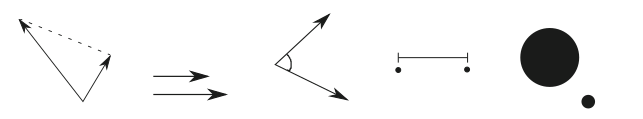
\includegraphics[scale=0.5]{img/simmeasures.png}
	\caption[Similarity measures]{\small{MultiMatch similarity measures: \textbf{Shape}: Vector difference between aligned scanpaths, normalised by 2x the screen diagonal. \textbf{Length}: Difference in vector lengths, normalized by the screen diagonal. \textbf{Direction}: Angular distance between saccade vectors, normalized by $\pi$. \textbf{Position}: Position difference of fixation, normalized by the screen diagonal. \textbf{Duration}: Duration differences of aligned fixations, normalized against maximum duration within the comparison.}}
	\label{fig:simmeasures}
\end{figure}


\begin{algorithm}[H]
	\begin{small}
		\SetKwInOut{Input}{Input}
		\SetKwInOut{Output}{Output}
		
		\Input{nx3 fixation vectors (x, y, duration), simplification thresholds $T_{Amp}$, $T_{Dir}$, $T_{Dur}$}
		\Output{eventfile: onset of scanpath, duration, and five similarity measures range [0, 1]}
		\For{\textbf{each} fixvector}
		{ 
			\For{\textbf{each} fixation \textit{f} in fixvector}
			{
				fixation$_x$, fixation$_y$, fixation$_{dur}$ = $x, y, duration$ \;
				saccade$_{x(y)}$ = fixation$_{x(y)}$$_{f}$ $-$ fixation$_{x(y)}$$_{f+1}$ \;
				saccade$_{lenx(leny)}$ = fixation$_{x(y)}$ $-$ saccade$_{x(y)}$\;
				saccade$_{rho}$, saccade$_{theta}$ = cartesian2polar(saccade$_{lenx}$, saccade$_{leny})$ \;
				\textbf{eyedata} = [fixation$_x$, fixation$_y$, fixation$_{dur}$, saccade$_x$, saccade$_y$, \newline saccade$_{lenx}$, saccade$_{leny}$, saccade$_{rho}$, saccade$_{theta}$]
			}
			\While{simplification is still possible}
			{
				\For{\textbf{each} saccade i in eyedata}
				{
					\If{angle(saccade$_{i}$, saccade$_{i+1}) < TDir$ \bfseries{and} $fixation_{dur} < TDur$}
					{combine saccades}
					\If{saccade$_{rho}$\space$_i$, saccade$_{rho}$\space$_{i+1}$) < TAmp \textbf{and} fixation$_{dur}$ $<$ TDur}{combine saccades}
				}
			}
		}
		\For{\textbf{each} pair of (simplified) scanpaths $S1 = \{u_1, \ldots, u_m\}, S2 = \{v_1, \ldots, v_n\}$}
		{
			calculate M: Matrix of saccade length differences between each $i \in S1$ and  $j \in S2$\;
			create a directed graph with elements of M as weights $w_1, \ldots, w_i$\;
			align scanpaths with $min(\sum w)$ from $M(0,0)$ to $M(n,m)$ via Dijkstra algorithm\;
			
			add aligned scanpath to set of aligned scanpaths \;
			
			\For{\textbf{each} pair($u_i,v_i$) in aligned scanpaths}
			{
				angular difference = angle($u_i, v_1$)\;
				position difference = $\sqrt{(x(u_i) - x(v_i))^2 + (y(u_i) - y(v_i))^2}$ \;
				vector difference = $\sqrt{(len\_x(u_i) - len\_x(v_i))^2 + (len\_y(u_i) - len\_y(v_i))^2}$\;
				length difference = $abs(rho(u_i) - rho(v_i))$\;
				duration difference = $abs(dur(u_i)-dur(v_i))$ \;
			}
			normalize angular difference by $\pi$\;
			normalize vector difference by 2x the screen diagonal (max theoretical distance)\;
			normalize length difference, position difference by the screen diagonal\;
			normalize duration difference by maximal duration difference in the scanpaths\;
			\textbf{sim\_measures} = median of each similarity measure\;
			\textbf{return} \textbf{sim\_measures}
		}
		\caption{multimatch}
		\label{algo:multimatch}
	\end{small}
\end{algorithm}

\subsubsection{multimatch usage in the studyforrest dataset}\label{sec:multimatch_forrest}
The use of the algorithm with the eye tracking data as provided in the REMoDNaV outputs required the implementation of some additional functions.
The extraction of eye events further included several considerations based on findings and known caveats in eye-tracking and attention research with dynamic scenes. The following section briefly describes these findings and the additional functions to accommodate them. For the main part, those functions are concerned with automatic scanpath extraction from the approximately 15 minutes spanning and several eye-movement categories containing eye-tracking event files by user-defined rules. In general, the functions ingest REMoDNaV result files as input, and output the fixation vector structure required by the MultiMatch algorithm. An overview in pseudocode can be found in algorithm \ref{algo:multimatch_forrest}. \newline
First, as the stimulus was dynamic, the start and end of pursuit movements were relabeled as fixations. This was done to accommodate the fact that most areas of interest in a movie are in motion. Focusing on the running young Forrest for example would likely appear as a slow pursuit in the eye event data. Disregarding such pursuits would lead to a large loss in data and variability, and as such, they were included via relabeling. \newline A different consideration concerned the selection of scanpaths from the approximately 15 minute long segments, as they are unsuitably long to derive a continuous attention measure or do a scanpath comparison on. It has been shown that subjects gazes have a bias towards the center in Hollywood movies (\cite{tseng2009quantifying}). This bias can at least in part be traced back to a strong center bias directly after cuts in dynamic scenes. \textcite{carmi2006visual} found the highest degree of exogenous attentional control (i.e. maximal inter-observer similarity in gaze as recorded via eye-tracking) in a moving collage of 50 heterogeneous video clips directly after cuts to new, semantically unrelated scenes. Without isolating cuts it therefore can not be disentangled whether the contribution of visual features of the movie on scanpaths stems from exogenous control from a movie element or from the sudden occurrence of a new scene after a cut. To not introduce such a confound in the similarity measures, the data was cut into segments that did not contain cuts to different scenes, relying on the location annotation by \textcite{hausler2016annotation}. The location annotation contained a detailed description of the timing of each of the 870 \textit{shots }of the movie (defined as a movie sequence between two cuts) as well as information about the depicted location in different levels of abstraction. In a first step, all consecutive short shots to the same locale (e.g. two consecutive, short movie shots in Forrest's bedroom, without any cuts containing semantically unrelated content) were grouped together. In this analysis, a “short” shot was defined as being shorter than the median length of 4.92s. This procedure increased the median length of shots from 4.92s to 7.019s. These elongated shots are henceforth referred to as \textit{snippets}. In a next step, within the scanpath comparison, the onset and offset times of the resulting snippets were extracted for every snippet longer than 4.92s. To not introduce an influence of snippet length into the similarity results, as longer movie snippets will be more likely to be less similar than short ones, scanpath lengths were standardized to approximately 4.92s seconds (the original median length). To further evade any problems associated with the center bias, scanpaths were extracted from the end of the snippet: The last oculomotor event within the range of the snippet marked the end of a scanpath. As such, scanpaths began maximally distant to the snippet onset.
As the eye movements of participants are interindividually different and do not correspond exactly to snippet timing, the precise onsets and resulting exact durations were computed as well, and stored for later use as regressors. The results of this computation can be found on Github\footnote{https://github.com/AdinaWagner/multimatch\_forrest} as well.\newline
\medskip

\begin{algorithm}[H]
	\begin{small}
		\SetKwInOut{Input}{Input}
		\SetKwInOut{Output}{Output}
		
		\Input{REMoDNaV eye movement datafiles per run, movie location annotation per run, desired length to elongate shots to \textit{ldur}, desired scanpath length \textit{dur}}
		\Output{One n x 3 fixation vector (x, y, duration) for any snippet longer than $dur$}
		{
			\If{$event_{row}$ = pursuit}
			{
				regard start and end points of pursuit as fixation
			}
		}
		\For{\textbf{each} row in REMoDNaV datafile}
		{
			\If{$event_{row}$ = fixation}{
				extract x-, y-coordinate, duration}
			\If{x, y < 0 or x > 1280 or y < 720}{discard as out-of-bound gaze}
		}
		\For{\textbf{each} row in annotation}
		{
			\If{($locale_{row} = locale_{row+1}$) and ($duration_{row}, duration_{row+1} < ldur$)}
			{combine to one shot}
		}
		\For{\textbf{each} row in annotation}
		{
			\If{$duration_{row}$ > dur)}
			{extract shotonset and offset time}
		}
		\For{ \textbf{each} i in length(onset)}
		{fixvector$_i$ = REMoDNaV[REMoDNaV$_{onset} > onset_i$; REMoDNaV$_{onset}$ < offset$_i$]
		}
		return $\{$fixvector$_1$, \ldots, fixvector$_i$$\}$, onsets, durations
		\caption{The studyforrest specific functions of multimatch}
		\label{algo:multimatch_forrest}
	\end{small}
\end{algorithm}

\subsection{A measure of attentional modulation from multimatch}\label{section:multimatch_attention}
A common measure of attentional modulation was computed in a two-step procedure. First, scanpath comparisons of all scanpaths from the same shot of two subjects were calculated for all possible pairs of subject. This resulted in $C_k(n) = {N\choose k} = {15\choose 2} = 105$ combinations for N = 15 subjects. These comparisons were done without any further simplification (i.e. no use of the direction, length, and duration thresholds), as even minor differences in scanpaths obtained from a movie can correspond to major differences in attended visual stimuli. In a second step, the resulting similarities for each of the five similarity dimensions, the onsets, and durations were averaged across subject comparisons, but within snippet. Thus, for each snippet longer than 4.92s five similarity measures were computed that represented the average similarity of scanpaths of all subjects on the given dimension. For further use in the functional ROI specificity analysis, the multimatch results were z-scored.
 
\subsection{ROI specificity of the FEF}\label{c3:FEF}

To combine all previous efforts, in a first step, the movie groupdataset was extended by including the FEF masks generated in chapter \ref{c2}. In a next step, the multimatch measures were included as event regressors into the glm computation. The z-scored similarity per dimension was used as the 'amplitude' of the event. As for its previously robust results, the Gaussian Naive Bayes algorithm was used during classification. The reasoning behind the analysis is the following: Higher similarity values in multimatch indicate greater exogenous attentional control evoked from the movie stimulus. If this continuous attentional mode modulates the left and right FEF differentially, this should be visible in the sign of the beta coefficient. \textbf{combine this with the hyptothesis of chapter 1} Initially, during conceptualization of the analysis, all five similarity measures were supposed to be included. The computation of the similarity results revealed a suboptimal correlation structure within the multimatch measures, though (further explored in section \ref{sec:res_mm}). As evident in figure \ref{fig:dist_hist}(c), only a maximum of two dimensions are simultaneously mutually uncorrelated. In linear regression, multicollinearity of regressors as introduced by such high correlations is undesirable, as the resulting regression coefficients would be highly unstable (\cite{wickens2014geometry}). To prevent this, two barely correlated ($r = -.12$) dimensions were sub-selected for the analysis, duration and position.  \\
\textbf{maybe put this into the discussion?}The position dimension indicates the similarity with regard to points of interest in the movie: Do participants fixate the same parts of the screen? The duration dimensions on the other hand may be more indicative of employed exploration strategies: Do participants fixate points of interest similarly long?


\section{Results}

\subsection{Eye movements and multimatch}\label{sec:res_mm}


Based on the REMoDNaV output, the multimatch method was able to extract a total of N = 533 scanpaths from the movie. The median duration of extracted scanpath duration was 4.39 seconds (mean = 4.36s) (see figure \ref{fig:dist_hist}). The median and average similarities per dimension are stated in table \ref{table:sims}.
\begin{table}[H]
	\centering
	\begin{tabular}{lC{3cm}C{2cm}C{3cm}}
		\thickhline 
		\textbf{Variable}	& \textbf{mean} [SD] & \textbf{median}  \\ \hline
		Vector similarity 	& $0.97$ $[0.01]$   & $0.97$  \\
		Position similarity	& $0.88$ $[0.03]$   & $ 0.89$  \\			
		Length similarity	& $0.96$ $[0.01]$   & $0.96$   \\			
		Duration similarity & $0.54$ $[0.05]$   & $0.55$  \\
		Direction similarity	& $0.72$ $[0.05]$ 	& $0.71$  \\ \thickhline
		\caption{Characteristics of scanpath similarity across the movie.}
		\label{table:sims}
	\end{tabular} 
\end{table}


%\begin{table}
%	\begin{center}
%		\begin{tabular}{C{2cm}C{2cm}C{2cm}C{2cm}C{2cm}C{2cm}}
%			\thickhline
%			& \textbf{Vector} & \textbf{Direction} & \textbf{Length} & \textbf{Position} & \textbf{Duration}  \\
%			\textbf{Vector} & 	- & $0.12$ & $0.97$ & $0.74$ & $-0.05$ \\ 
%			\textbf{Direction} & **  & - & $0.15$ & $0.04$ & $0.72$ \\
%			\textbf{Length} & *** & *** & - & $0.72$ & $0.04$ \\
%			\textbf{Position} & *** & n.s.	 & *** & - & $-0.12$ \\
%			\textbf{Duration } &  n.s.	& *** & n.s. & ** & - \\ \thickhline
%		\end{tabular}
%	\end{center}
%	\footnotesize Significance codes: *** $p < 0.001$, ** $p < 0.01$, * $p < 0.05$
%	\caption{Pearson correlations of similarity metrics}
%	\label{table:correlations}
%\end{table}



Figure \ref{fig:dist_hist} gives an overview of some additional scanpath characteristics, in particular the distribution of similarity per dimension, the onset of scanpaths in the first run, and an example of movie segments with high and low similarity.

\begin{figure}[H]

	\subfigure[Extracted scanpathlengths]{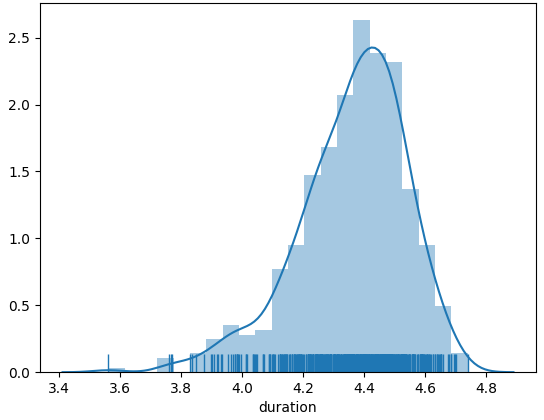
\includegraphics[width=0.5\textwidth]{img/dist_hist_v2.png}}
	\subfigure[Distribution of similarities per dimension for the movie]{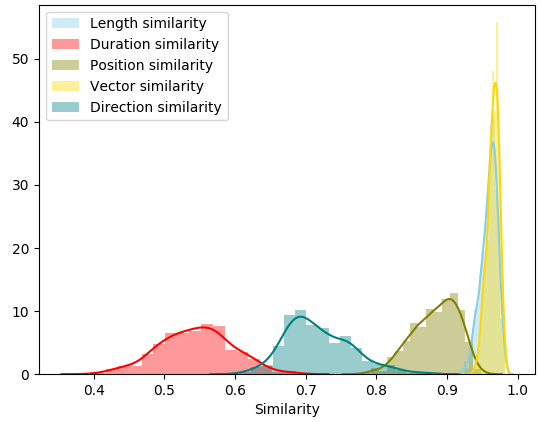
\includegraphics[width=0.49\textwidth]{img/sim_per_dimension_v2.png}}
	\subfigure[Correlation heatmap between dimensions]{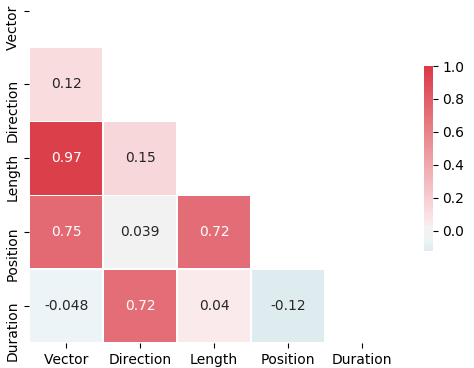
\includegraphics[width=0.49\textwidth]{img/sim_corr_v2.png}}
	\subfigure[\textbf{TODO: one more plot for prettiness}]{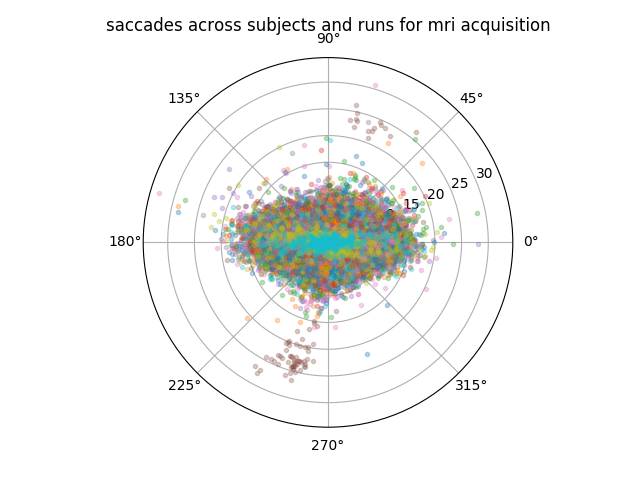
\includegraphics[width=0.49\textwidth]{img/mri_all_saccades.png}}
	\subfigure[Average onsets of scanpaths in seconds for the first run]{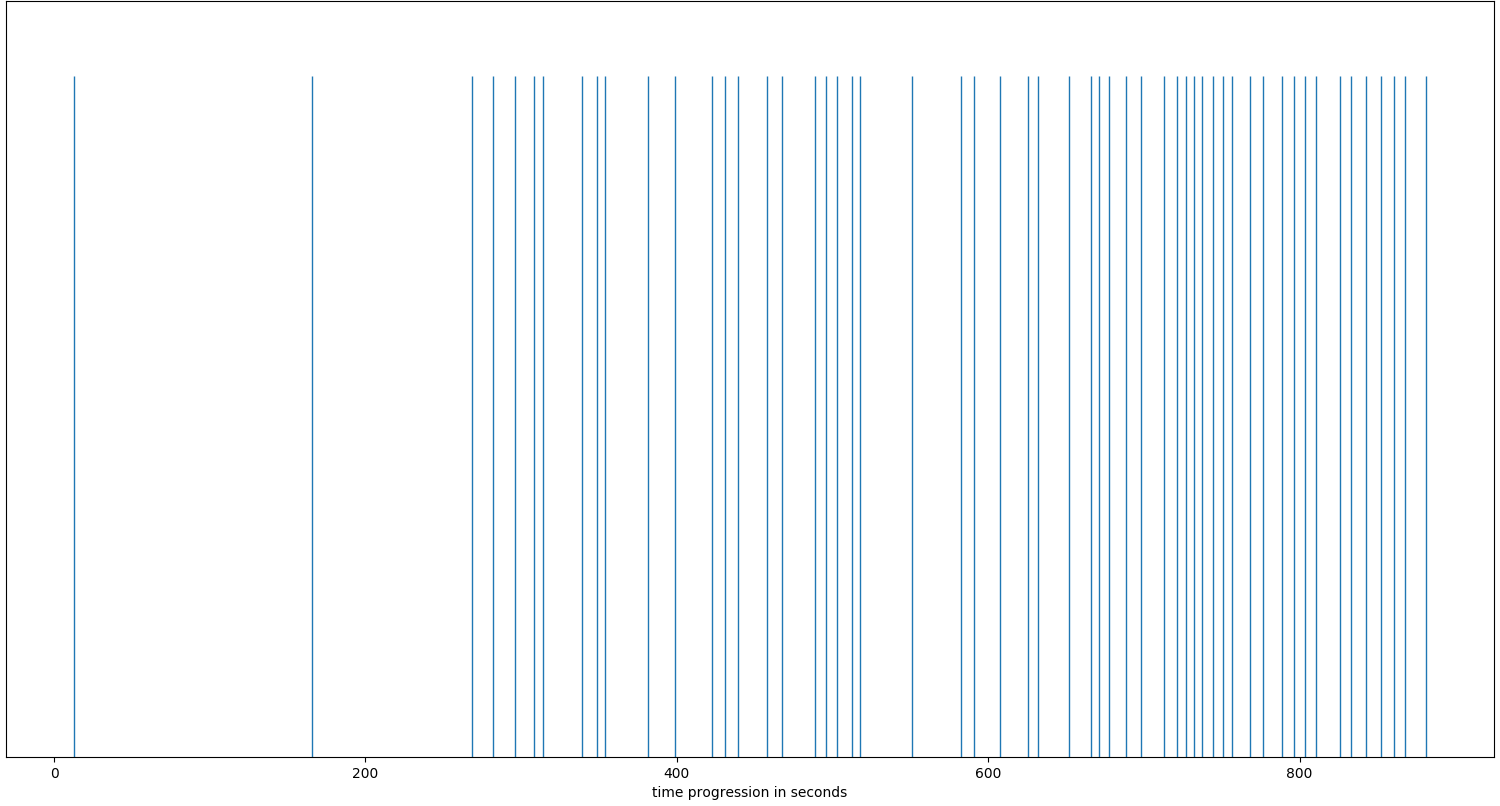
\includegraphics[height=50pt, width=1\textwidth]{img/scanpath_onsets_v2.png}}
	\subfigure[Frame from movie snippet with the lowest average similarity rating of run 1, with overlaid eyegaze]{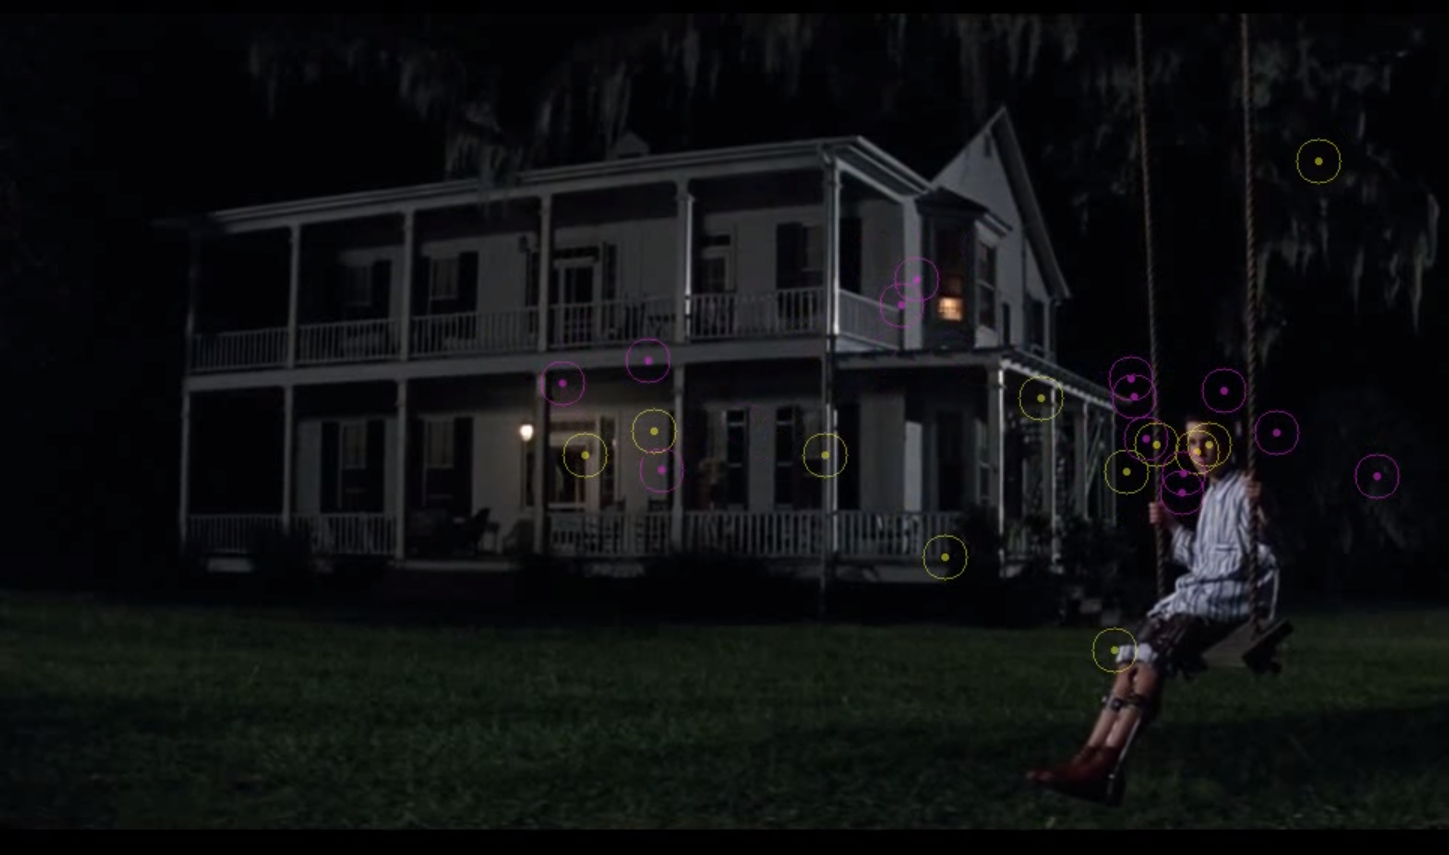
\includegraphics[height=0.18\textheight, width=0.49\textwidth]{img/low_sim.png}}
	\subfigure[Frame from movie snippet with the highest average similarity rating of run 1, with overlaid eyegaze]{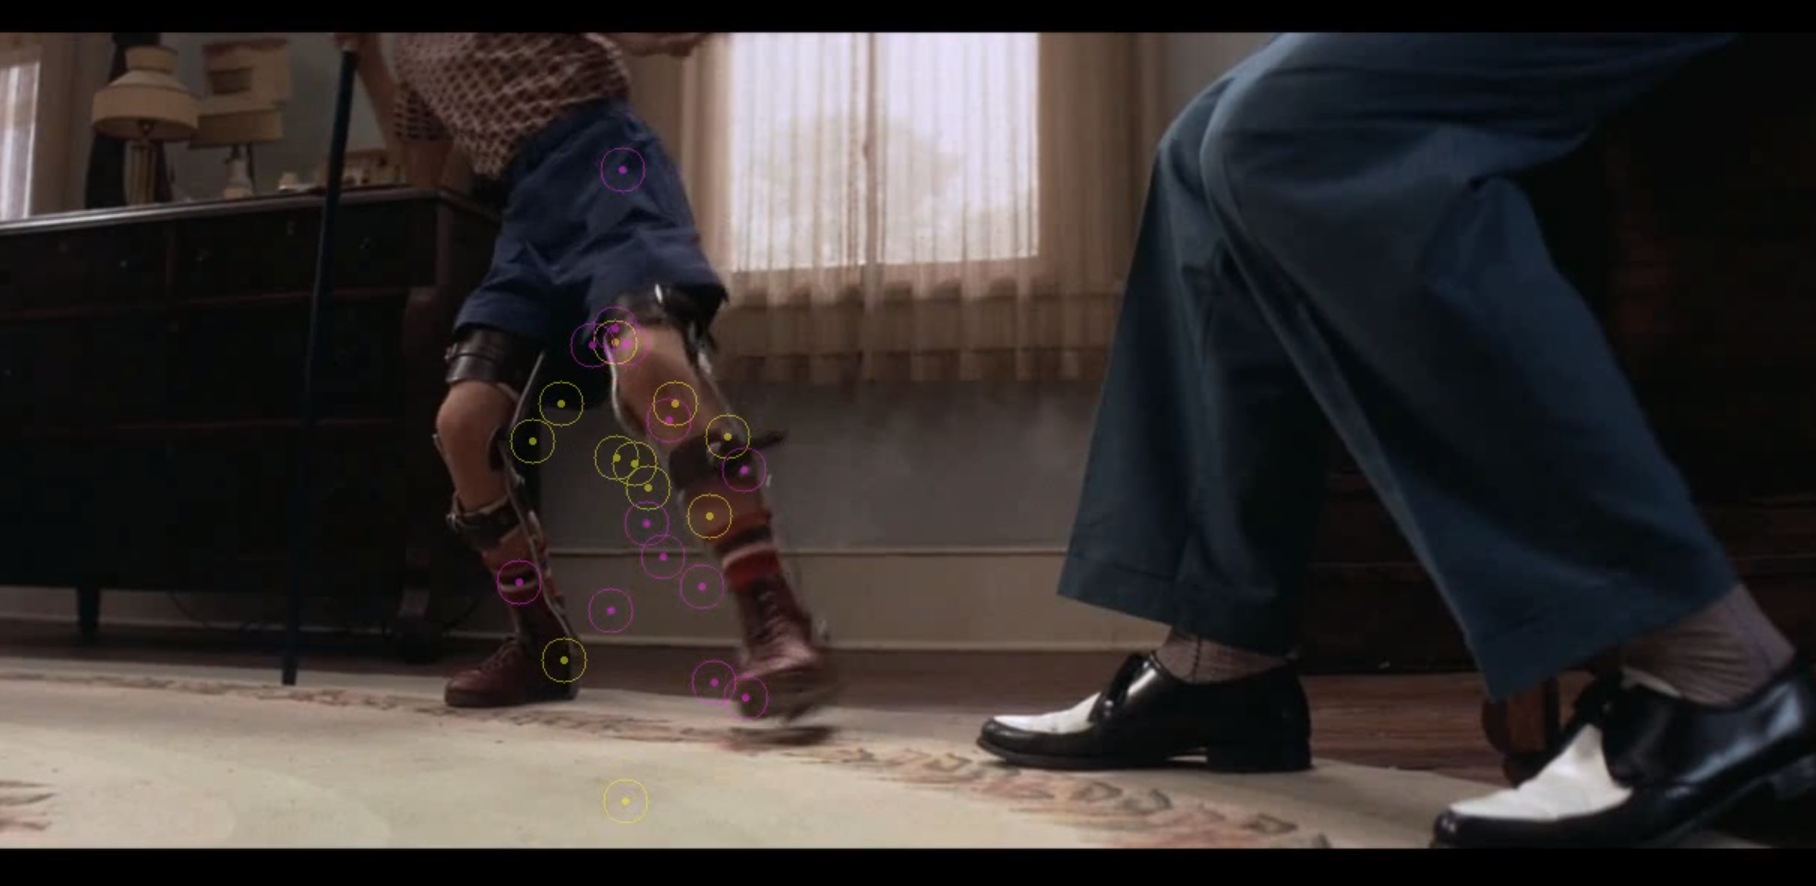
\includegraphics[height=0.18\textheight, width=0.49\textwidth]{img/max_sim.png}}
	\caption{\small{Overview of extracted scanpaths' characteristics.}}
	\label{fig:dist_hist}
\end{figure}

\subsection{ROI specificity of the FEF}

Figure \ref{fig:CV_FEF} shows the classification performance of the GNB during the classification step. Depicted are classification results for a dataset in which ROIs are combined across hemispheres (bilateral ROIs), and one in which the hemisphere information is preserved (lateralized ROIs). 

\begin{figure}[H]
	\subfigure{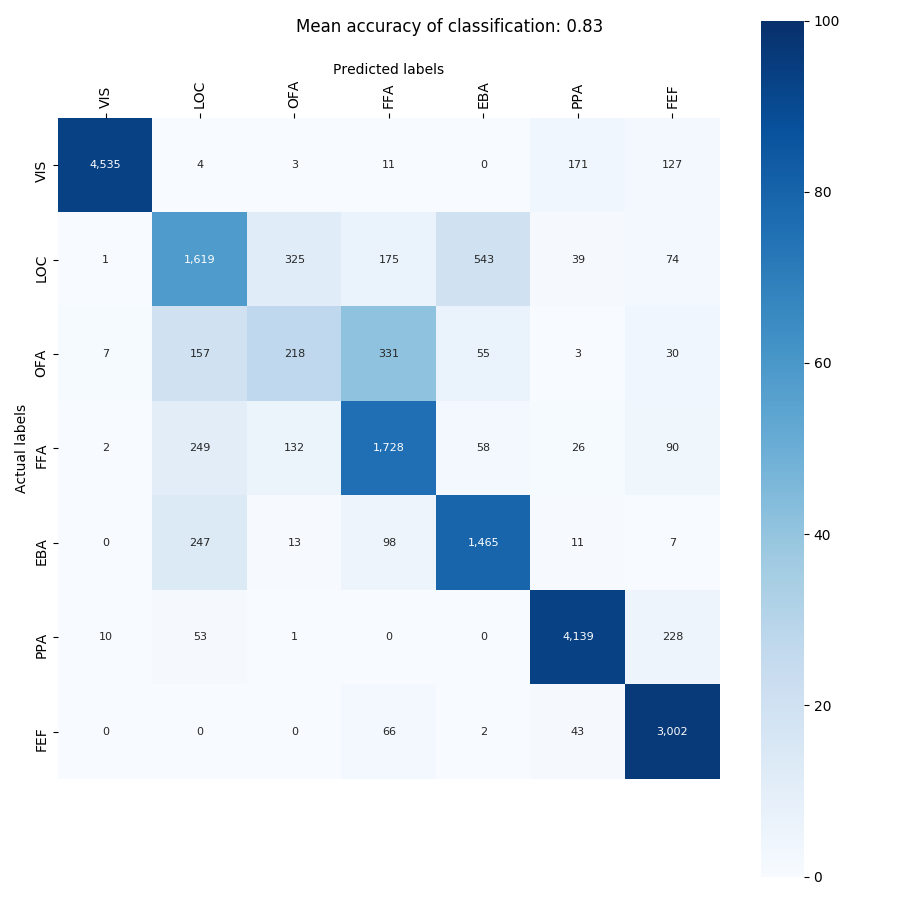
\includegraphics[width=0.49\textwidth]{img/FEF_CV_lat.png}}
	\subfigure{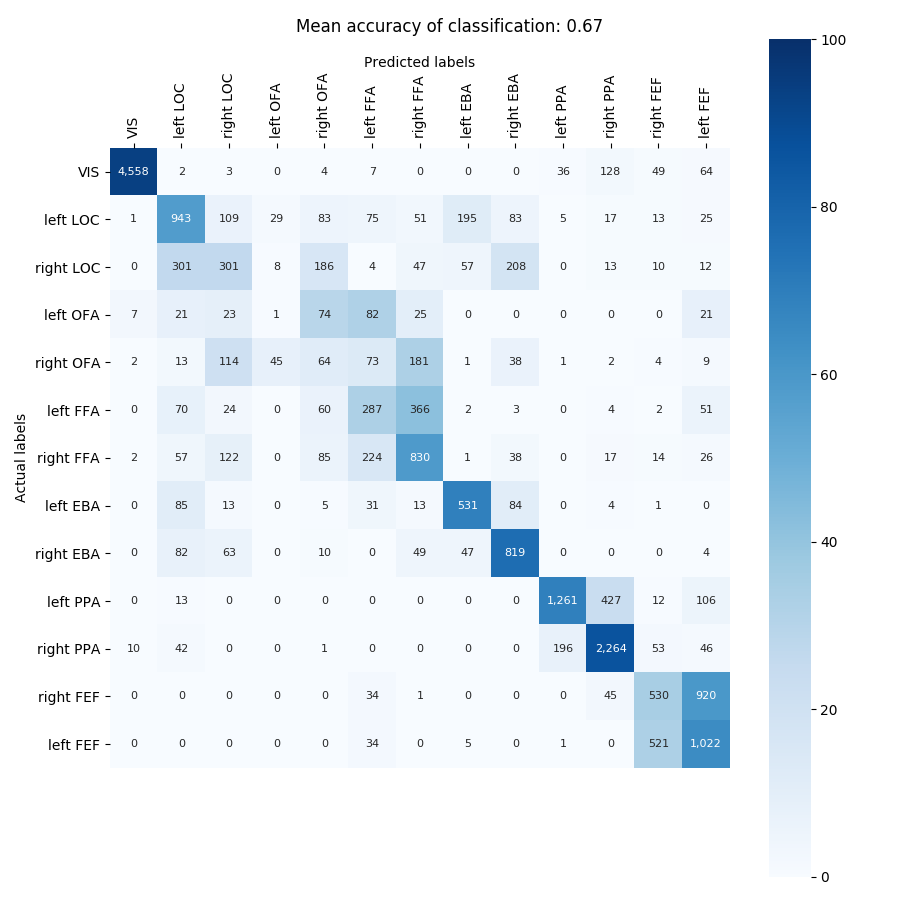
\includegraphics[width=0.49\textwidth]{img/FEF_CV_bilat.png}}
	\caption[Classification results with the FEF]{{\small Confusion matrices displaying the classification performance for all ROIs including the FEF for a dataset with bilateral  (left) and lateralized ROIs (right). Color shows classification accuracy (from 0 to 100\%) while numbers in each cell correspond to the actual number of voxels	across all subjects.}}
	\label{fig:CV_FEF}
\end{figure}

Figure \ref{fig:tc_FEF} shows the GLM results for the time course of sensitivities in the ROI pair left FEF and right FEF for the first run of the movie data. Positive sensitivities correspond to differentially higher left FEF activation, and negative sensitivities correspond to differentially higher right FEF activation. The color bars correspond to the two multimatch measures, and their width indicates the length of the scanpath over which the similarity measure was calculated. Color bars only display the duration of the regressor, but not its amplitude. As evident from the graph, the variability in hemispheric activation differences in the FEF was not explained with the available multimatch data (R$^2$ = 0.03).

\begin{figure}[H]
	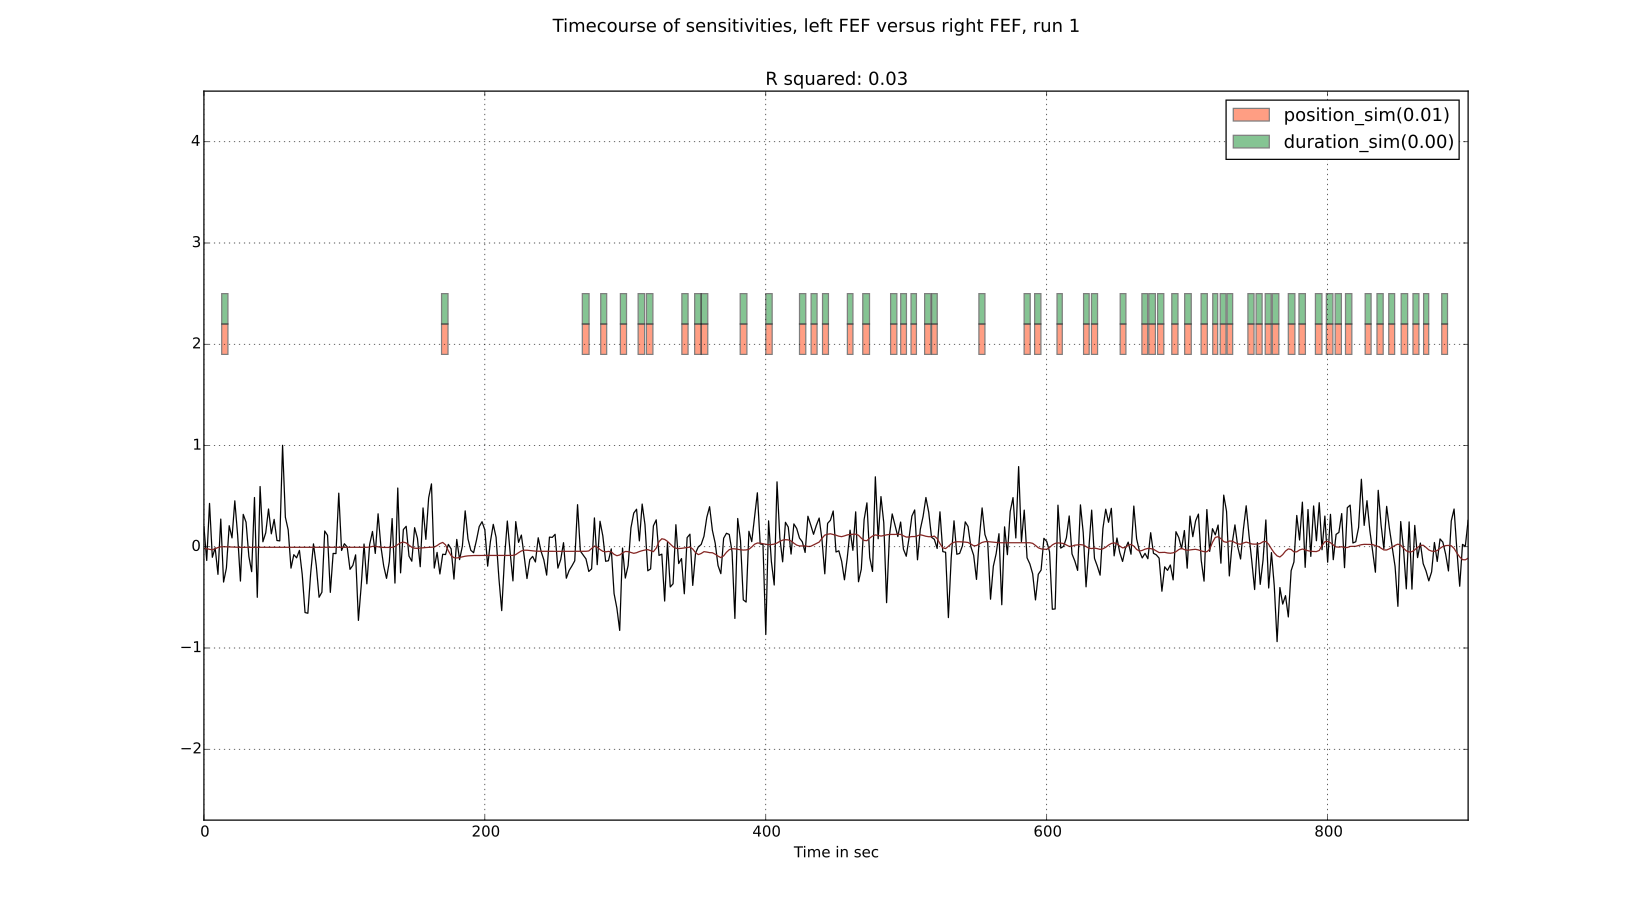
\includegraphics[scale=0.3]{img/tc_lFEF_rFEF.png}
	\caption[short text]{{\small Functional specificity of left and right FEF during run 1. Black line: Sensitivities derived from classification with a linear GNB. Red line: GLM fit from regressing sensitivities onto the multimatch results. Colors correspond to the regressors, widths indicate the scanpath length. Beta values are given in brackets.}}
	\label{fig:tc_FEF}	
\end{figure}


\section{Discussion}


\subsection{multimatch}
The implemented multimatch algorithm was able to extract scanpaths and calculate their similarity on five different dimensions. The average length of extracted scanpaths was shorter than the duration aimed at (4.92s), as the onset and offset of the required eye movements did rarely correspond exactly to the onsets and offsets of the selected movie snippet. Nevertheless, the extracted scanpaths were similar in duration (also visible from the regressor color bar widths in figure \ref{fig:tc_FEF}), and hence do not introduce a bias of scanpath lengths into the similarity calculation. With the exception of the movie start with three very long shots, the extracted scanpaths are distributed evenly across the movie. As evident from table \ref{table:sims} and figure \ref{fig:dist_hist}, scanpaths were almost perfectly similar on the dimensions vector length and vector position. This is likely at least partially due to the scanpath alignment based on the scanpath shape. Scanpaths were also highly similar on the position dimension, which underlines the strong gaze control of the movie stimulus. Subjects scanpaths differed more substantially on the dimensions direction and duration, which indicates differences in fixation dwelling times and saccadic angle. Thus, the general points of interest (as evident from high similarities in position, length and shape) were similar across subject, but differences in direction and duration might indicate interindividually different exploration strategies. All dimensions show a remarkable consistency in similarity measures as evident from the small standard deviations. Following the reasoning behind the implementation of the method, this might indicate a consistently high level of exogenous control by the movie stimulus. This finding is consistent with research on viewing behavior during movies: Unlike during static image viewing, the spatio-temporal gaze behavior of multiple viewers exhibits a substantial degree of coordination in movie watching. \textcite{smith2008attentional} cued the term \textit{attentional synchrony} for this phenomenon. During attentional synchrony, viewers gazes cluster around a small portion of the screen at any one moment. \textcite{goldstein2007people}, for example, found the distribution of fixations of viewers to occupy less than 12\% of the total screen area in more than 50\% of the time in six Hollywood movies. In a comparison between different types of static and dynamic visual stimuli, \textcite{dorr2010variability} found the highest consistency between viewers eyegazes during professionally produced (Hollywood) movies, likely largely due to the use of cinematic composition of scenes, deliberate camera work and editing. Hasson, Yang et al., 2008 found high correspondence in gaze behavior across subjects, even for backwards presentations of movies. \newline

\subsection{ROI specificity of the FEF}
The classification results in figure \ref{fig:CV_FEF} show that a classification of voxel into ROIs is also possible for the obtained FEF masks. Misclassifications into ROIs of higher visual areas are very rare. The FEF therefore seem to show an activation pattern that is well distinguishable from other ROIs, and similar across participants. The same classification analysis on hemisphere specific ROIs shows, though, that a classification into left and right instance of the ROI is more difficult in the case of the FEF. While areas such as the right and left EBA or the right and left PPA are well distinguished by the classifier, this is not true for the left and right FEF. Note that this should not influence the sensitivities used in the GLM negatively - the feature weights are derived during training, the classification results stem from testing. However, this does show that activation patterns between left and right FEF are not well distinguishable for this classifier. However, the classification accuracy for lateralized ROIs decreases in general compared to the classification analysis with bilateral ROIs (accuracies of .67 and .83, respectively), and the FEF is not the only ROI in which left and right hemisphere are not well classified (see performance for FFA and LOC).\\
As the time course of sensitivities (black line in fig \ref{fig:tc_FEF}) shows, there are activation differences in the right and left FEF over the course of the movie. The attentional mode measure as computed with multimatch was not able to explain these differences, though. Both regressors have a beta weights of essentially zero, and the explained variability is similarly low. \\
This result can have several reasons. Arguing in the same perspective as the derivation of the analysis, this result could indicate that there is no differential attentional modulation between the left and the right FEF. However, the complexity of this analysis, and the multitude of assumptions that underlie individual computation steps, could not permit such a conclusion, and potential problems should be discussed in depth. One possibility are practical and theoretical deficiencies in the multimatch regressors. For one, as discussed in the previous section, their variability is extremely low. Even though the position and duration dimension differ in their absolute values, the similarities within one dimension have a very low standard deviation. This reduced variability decreases the use of the measure as a regressor. A computation of scanpath similarities for longer time periods could potentially increase the variability, but resulting scanpaths would include cuts and the results of this approach would thus be affected by the caveats outlined in section \ref{section:multimatch}. Secondly, however, the consideration of cuts and scenes prevented a continuous attention mode measure. Especially long scenes as in the beginning of the movie are not captured in the regressor. Further, as evident in figure \ref{fig:tc_FEF}, the sensitivities follow a time course that appears to be more fine-grained than the roughly 5 second long multimatch events, indicating that a measure of greater temporal resolution would be necessary to model the activation differences. Lastly, concerning the potentially weakest assumption of this thesis, it could be questioned whether attentional mode can be derived from eye gaze during movie watching. As evident from the consistency in scanpath similarity, the MultiMatch method was not able to detect large changes in attentional mode throughout the movie. This might reflect a consistently high exogenous control exercised by the movie stimulus. However, it is not clear whether similarity in scanpaths does actually correspond to exogenous control. The similarity measures obtained from eye gazes could fail to differentiate exogenous modulation from endogenous influences arising from a shared goal between participants. Consider the following example: in order to fully comprehend the movie content, it might be of relevance for every subject to endogenously focus on the facial features of Forrest in his dialogue with Jenny. This scene does not contain salient stimulus features or other types of exogenous control, yet it would lead to a high similarity measure. A high degree of synchrony in eye movements therefore would not necessarily correspond to purely exogenous influences. Thus, it remains questionable whether the regressor can capture attention mode differences both due to low variability in the measures and unclear differentiability of said measures with eye gaze similarity, at least during Hollywood movies. \textcite{dorr2010variability} found more variability and subject-specific idiosyncrasies in other types of dynamic natural scenes, such self-recorded videos of pedestrian zones. \textbf{therefore those might be a better stimulus choice.,,,}A more thorough investigation of the origin of eye gaze similarity might lie in a subsequent qualitative analysis of individual movie shots, but that was not within the scope of this thesis. \\
One possibility to get closer to an answer about whether activation differences contain variability that could be attributable to attentional modulation is to approach the problem from another angle: A sensible first step may be to investigate whether there are any activation differences beyond those induced by eye movements in the first place. As evident from the sensitivity time course, there are clear activation differences, and it might be interesting to see whether these can stem solely from eye movements. In principle, the sensitivities entered into the glm are averaged across folds of the cross-validation. Individual FEF activation patterns from unconstrained eye movements of individual participants to different directions at the same time point could thus average each other out. However, the literature suggests and the multimatch results confirm a remarkable consistency in gaze behavior during movie watching. Common patterns such as the aforementioned centering of gaze after cuts, or very salient events in the periphery of the screen could thus indeed be captured in the sensitivities. One possibility to investigate this hypothesis is to use an averaged saccade regressor for the horizontal plane. Leftward saccade amplitudes could be given a negative sign, and rightward saccades a positive sign. If the averaged amplitudes of saccadic eye movements of all participants within a certain time frame, for example per second, differ from zero, a majority of participants performed a saccade in the same (left or right) direction at this point of the movie. Such a regressor would have a greater temporal resolution, and including in into the analysis could shed light on whether observed activation differences indeed only stem from eye movements, or whether there is remaining activation that could potentially stem from differential attentional modulation of the FEF between hemispheres.

\bigskip 

\textbf{TODO: explain reasoning behind multivariate nature of the classifier}

\chapter{General discussion}\label{section:discussion}
The aim of this thesis was to investigate the functional neuroanatomy of the visuospatial attention system with fMRI and eye tracking data obtained during naturalistic stimulation with a Hollywood movie. For this, I selected a particular part of the dorsal attention system, the frontal eye fields, and attempted to gain insights into the possible contribution of attentional mode to its distinction between the left and right hemisphere. \\
To conduct this analysis, I undertook a number preliminary analysis steps, and combined efforts from several software- and analysis sub-projects. This thesis, therefore, contains a dense collection of methodological advancements and analysis results: Chapter \ref{c1} contained the development of a novel method to determine functional ROI specificity and the results of two validation analyses. Chapter \ref{c2} involved the localization of the frontal eye fields with a GLM on unconstrained eye movements under natural stimulation with a Hollywood movie with fitlins. Using the MultiMatch algorithm, parts of chapter \ref{c3} dealt with the computation of a measure of similarity between scanpaths of participants for movie scenes in order to use the obtained results as a measure of attentional mode. Lastly, all of these efforts were combined to the functional specificity analysis in the section \ref{c3:FEF}. \\
The results show that the sensitivities, the averaged parameter vectors of linear decision hyperplanes in the binary classification of left and right FEF voxels into ROIs, can not be modeled with an attentional regressor build from scanpath similarities during movie watching. They did however show an interesting sensitivity time course, and uphold the question whether there is a cognitive contribution beyond the influence of motor functions in eye movement to the observed differences. Beyond the initial research question, the results obtained from the previous analysis steps provide methodological advancements. First of all, the validation analyses provide a general proof of principle for the ROI specificity method. This thesis therefore outlined a novel approach to gain insights into functional specificity of ROIs, and demonstrated its application with standard event files (localizer validation analysis), complex stimulus annotations (movie generalization), and behavioral measures (FEF analysis). Simultaneously, the results provide further evidence that ROI localization is possible with naturalistic stimulation. While most classification results presented in this thesis a linear Gaussian Naive Bayes classification algorithm, stochastic gradient descent also showed to be suitable. Even though this thesis used a GNB for easier interpretability of the decision boundary parameters, using an SGD is equally possible, and potentially more sound as for the fewer assumptions of this classifier. In the same vein, the results show that localization of the FEF with eye tracking recorded during naturalistic stimulation with a Hollywood movie is generally possible, but suffers from the center bias of Hollywood movies, that restricts the range of eye movements. Lastly, this thesis is a thorough example of how data from several modalities, BOLD data, eye tracking data, and stimulus descriptions, of a large dataset can be combined in a sensible manner. \\
Nevertheless, a number of potential issues need to be addressed to access the validity of the methods and results. As already discussed, the scanpath similarities computed with multimatch were very consistent. This corresponds to the literature on gaze behavior during movie watching. This however emerged as a practical constraint for the FEF specificity analysis. Furthermore, there are theoretical concerns whether the multimatch results can be mapped to attentional processes in the case of Hollywood movies with their strong guidance of viewing behavior. These limitations do not enable a confident rejection of hemisphere specific attentional modulation of the FEF. They did however point out improvements for future analyses of this question. With regard to the method validation and generalization of the ROI specificity approach, some words of caution need to be raised. This first part of the thesis was largely exploratory in regard to determining the functional specificity of chosen ROIs. This approach showed that the value and novelty of the developed method lie in its ability to explore previously unknown functions with naturalistic stimulation. As such, it is providing interesting and important new insights on the level of functional neuroanatomy. The results further constitute additional evidence that the use of naturalistic stimulation is of immense value in neuroimaging research and can underlie experimental control (\cite{hasson2004intersubject}). Nevertheless, any exploratory analysis is lacking a thorough derivation of hypothesis from theory, and the preregistration of such hypotheses to guarantee scientific integrity. Furthermore, given that the choices of annotation for naturalistic stimulation and their inclusion can potentially be unlimited, the method leaves many researchers degrees of freedom to potentially bend results into shape. Therefore, it is important to note that the method does not suffice on its own. Instead, it should be regarded as a valuable first step to gain exploratory insights and generate novel hypotheses. The ideas derived from the method should subsequently be brought to test on new data to prevent findings due to chance being published without further testing. Furthermore, the validation analysis of the ROI specificity method on the localizer data is \textit{circular}, as the classification is performed on the same data used to derive the higher visual area ROI masks. This practice is prone to give distorted descriptive and invalid inferential statistics, as voxel in test and training set are no longer independent (\cite{kriegeskorte2009circular}). However, for the analysis at hand, independence was achieved in the movie data, and the classification results appear to be robust. Nevertheless, the extraordinary cleanliness of the sensitivity time course in the localizer data is very likely at least in part an artifact from the subselection of voxel with activation related to the localization stimulation protocol during ROI selection. In the same vein, the derivation of FEF masks from movie data and subsequent ROI specificity with movie data can be considered problematic. To prevent this circularity, the method needs to be tested further. Two different possibilities for this arise in the near future. For one, the method could be used with any experiments data and a 'blind' ROI selection, for example utilizing the HCP-MMP1 multimodal cortical parcelation (\cite{glasser2016multi}), consisting of 360 parcels of the whole cortex. This parcelation is independent of voxel activation in the datasets, and could especially in the case of the movie experiment help to shed light on the functional specificities of unexplored regions during movie watching. Secondly, an Honors Thesis project concerned with a similar classification question based on a different movie dataset in the Haxby Lab has agreed to test the method on their new data after completion of the thesis. Therefore, the work undertaken in this thesis also constitutes a starting point for further development and future application of the method.
\\
Beyond its use in this mere Masters thesis, the work presented here has also led to more lasting, shared resources in the form of data, software, and methods, that can be used more widely in other scientific work. In the wake of the analysis, I contributed with code and discussions to PyMVPA (\cite{hanke2009pymvpa}), fitlins (\cite{markiewicz_christopher_j_2019_2555453}), pybids (\cite{yarkoni_tal_2019_2555449}) and REMoDNaV (\cite{dar2019}). Furthermore, I ported the matlab toolbox MultiMatch (\cite{dewhurst2012depends}) into the pip-installable Python module multimatch and thus provided an accessible open source distribution of a closed software program that can easily be advanced further with the collaborative development possibilities of Github. This might enable additional research into scanpath similarity with this geometric, multidimensional approach, without requiring usage and purchase of closed source software. The ROI specificity method has been submitted as an abstract to the OHBM, and can thus hopefully be presented to and discussed with a broader scientific audience. Lastly, the scanpath similarity data during movie watching has been publicly shared on Github, as well as all analyses code reported in this thesis. These first attempts to curate something within the scope of my abilities back to the research community in neuroscience were helpful for me in many ways. Sharing code or software encouraged me to document my work as best as I could. Visibility of the code and collaborations building up on it have been able to pinpoint errors I inadvertently made and will continue to do so in the future. Finding errors in others software, verifying that the error is not due to own mistakes, and filing issues or even finding fixes motivated me to understand programs instead of only using them. Finally, trying to give something back is the least I can do to contribute to the collaborative, friendly, and educational neuroscience/neuroinformatics community I experienced. Others' shared open data, open source software the analysis relied upon, or code and tutorials I could learn programming from, were the backbone of this thesis.



 \begin{itemize}
 	\item elaborate on the fact that everything reported here is basically descriptive, not inferential
 	\item make a point about how throughout analyses like this are only possible because of data sharing and open science, and open source software.
 \end{itemize}
 
 
 \bigskip 
 
  ....
 
 
\begin{itemize}
 	\item (maybe refer to Deborah Mayos Severe Testing ideas?)
 	\item Problem of 5 different similarity measures --- BUT successfully used by French et al., multidimensional construct preferable as might explain more variance (citation? check anderson or the other dewhurst publication) 
 	\item Address the question of whether the linearity and gaussian distribution assumptions hold.
 	\item Now trash all shortcomings and come to the conclusion that for was done and despite a number of limitations this thesis was able to advance the literature in the following ways
 	\item 
 	
\end{itemize}
 
 \bigskip
... Likewise, this thesis provided an example of how the eye tracking data of the studyforrest publication can be utilized in fMRI analyses....
\bigskip
 


\begin{itemize}
	\item Future: non-linear classifier?
\end{itemize}


\section{Conclusions}
\begin{itemize}
	\item now what have we all learned after reading this far?
	\item surely something needs additional research
	
\end{itemize}

\textbf{TODOs}

\textbf{small shit}
\begin{itemize}
	\item passive constructions
	\item long sentences
	\item verbal connections between sections. Short intros and outros of all main chapters.
	\item Citations
	\item all \textbf{bold} citations are not yet in bibtex
	\item Things are not optimally aranged currently, once the text is in final form make sure to force figures and algorithms to their appropriate places.
	\item captions for things in the lists of figures and tables.
\end{itemize}




\pagebreak

\bigskip\bigskip

\clearpage





%------- Literaturverzeichnis -------------------
%%%% Literaturverzeichnis macht aktuell Probleme, könnte bibtex unter Debian sein
\printbibliography[	heading=bibintoc,			% oder bibnumbered
										title={Bibliography},
										nottype=online]
%									]	
\nocite{*} % auch nicht zitierte Werke ausgeben									


%--------- alternatives Literaturverzeichnis -------
% so kann man das Literaturverzeichnis direkt erzeugen
% \begin{thebibliography}{99}
% \addcontentsline{toc}{chapter}{Literaturverzeichnis}
% \bibitem{nelsen}Nelsen, Roger B.: An Introduction to Copulas, Springer, Portland, 2006. 																											
% \bibitem{lindner}	Lindner,	Alexander:	Skript zur Wahrscheinlichkeitstheorie SoSe 2014,	Braunschweig,	2014.																																											
% \end{thebibliography}


\begin{appendices}
	
\chapter{Additional tables and graphics}\label{A:addons}

As for a subsequent descriptive investigation of the stimulus contents contributing to a FFA-PPA distinction, figure \ref{fig:scenes} shows the middle frames of scenes consistently, i.e. in all dataset sizes and classifier choices, associated with a high positive or high negative beta weight with overlaid eye gazes.
An in depth investigation of stimulus properties was not within the scope of this thesis, however, this short descriptive overview confirms general known functional specificities of the FFA and PPA. High betas correspond to scenes with dialogues or groups of people (as for the choir or in the football stadium). Low betas in turn show more associations with rural or urban scenes.

\begin{figure}[H]
	\subfigure{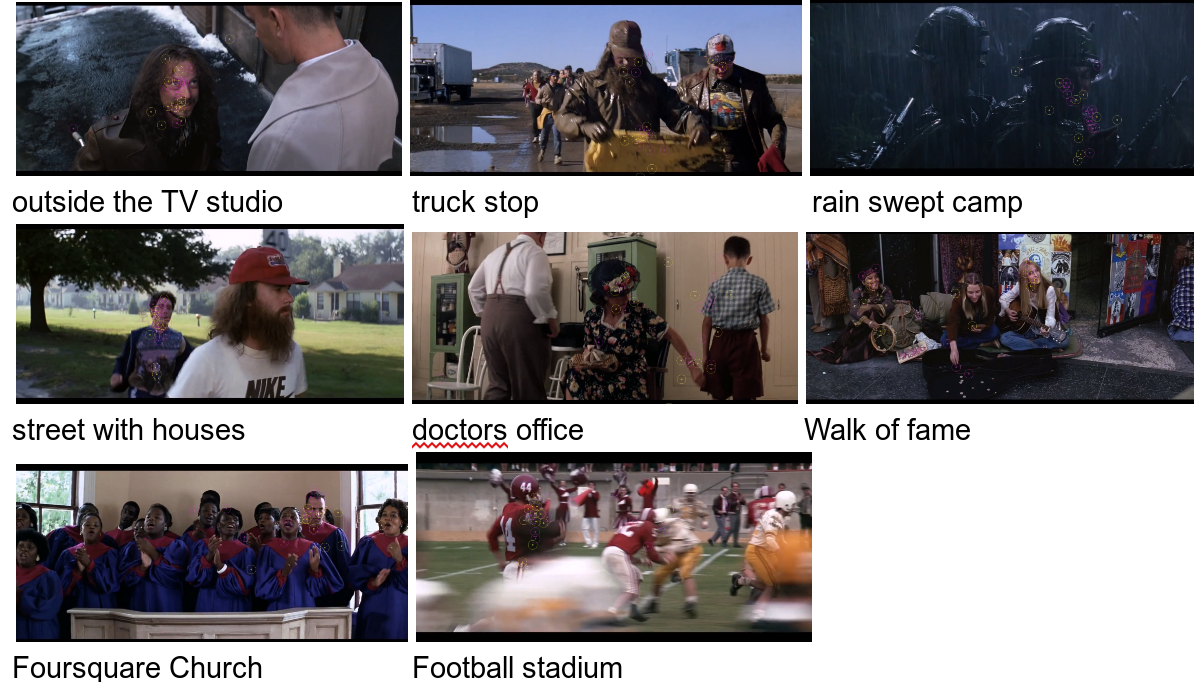
\includegraphics[scale=0.4]{img/highest_betaFFA.png}}
	\subfigure{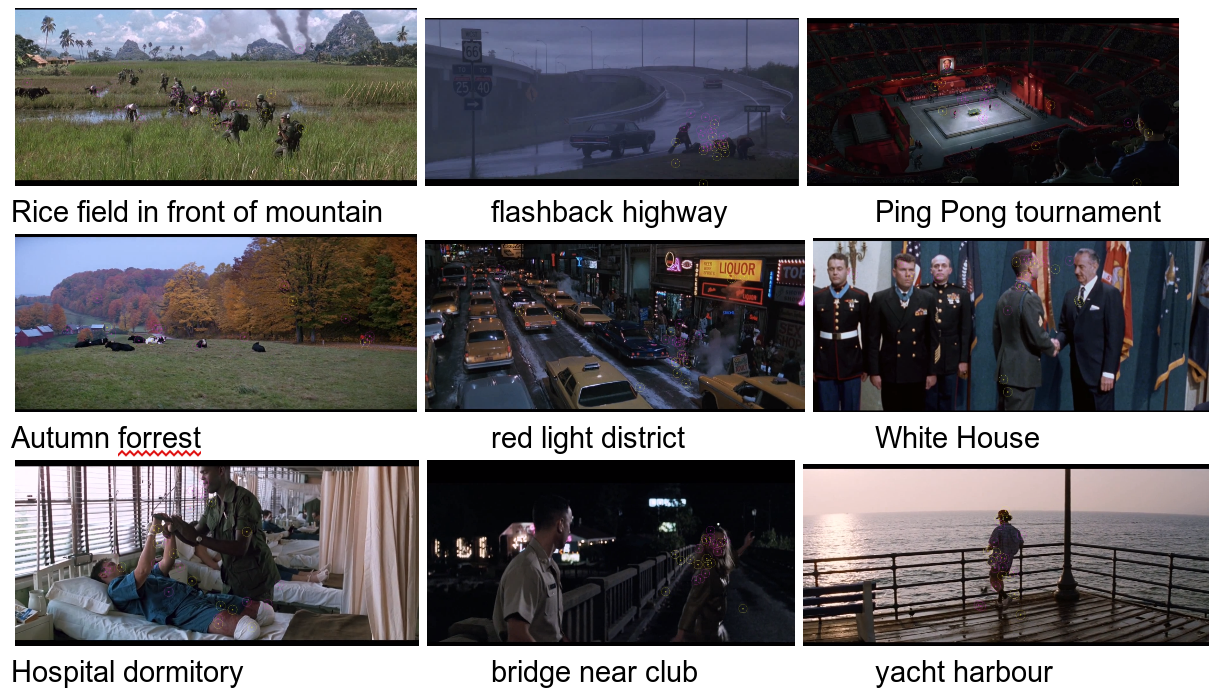
\includegraphics[scale=0.4]{img/highest_betaPPA.png}}
	\caption[Descriptive analysis of diagnostic scenes]{\small{Middle frame of scenes consistently associated with a high positive (top frame) or negative (bottom frame) beta value with overlayed eye-gaze (circles).}}
	\label{fig:scenes}
\end{figure}
	

\chapter{Code}\label{A:code}

\begin{figure} [H]
	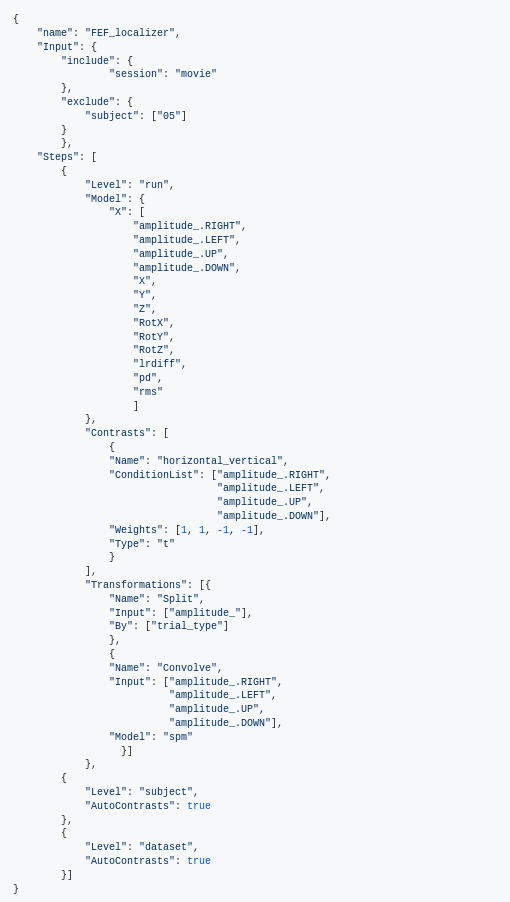
\includegraphics[scale = 0.7]{img/json_fitlins.png}\hfill
	\caption{json file with fitlins model specification}
	\label{A:fitlins}
\end{figure}



The model specified for fitlins follows the BIDS Extension Proposal 002 concerning statistical models\footnote{https://docs.google.com/document/d/1bq5eNDHTb6Nkx3WUiOBgKvLNnaa5OMcGtD0AZ9yms2M/edit}. The keyword \texttt{X} denotes the design matrix specification. For the first level of this analysis, as evident from the values supplied to the keyword, four directions of saccades, six motion parameters (X, Y, Z, RotX, RotZ, RotY) and three stimulus confounds (lrdiff, pd, rms) are used to build a design matrix. An example design matrix for one subject and run is shown in figure \ref{fig:des}. 
\begin{figure}[H]
	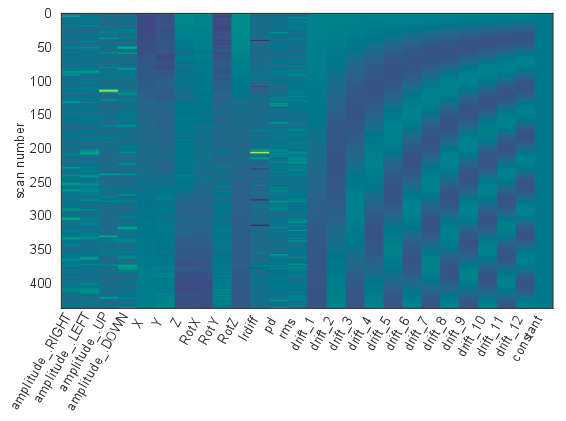
\includegraphics[scale=0.5]{img/ex_design.png}
	\caption{A firstlevel design matrix with fitlins}
	\label{fig:des}
\end{figure}

First level contrasts involve only the saccade directions and specify the \texttt{horizontal\_vertical} contrast. The first level transformations are \texttt{Split}, to obtain four saccade regressors and their amplitude\footnote{without this transformation, the amplitude information of the regressors would have been lost.}, and \texttt{Convolve}, to convolve the saccade regressors with spms HRF. The following analysis level, subject and dataset, carry the contrast through with fitlins \texttt{Autocontrast} function.



\end{appendices}




\end{document}